\documentclass[12pt,a4paper]{report}

% ??? PACKAGES ?????????????????????????????????????????
\usepackage[utf8]{inputenc}
\usepackage[T1]{fontenc}
\usepackage{babel}
\usepackage{geometry}
\usepackage{graphicx}
\usepackage{xcolor}
\usepackage{hyperref}
\usepackage{listings}
\usepackage{booktabs}
\usepackage{tabularx}
\usepackage{array}
\usepackage{longtable}
\usepackage{multirow}
\usepackage{fancyhdr}
\usepackage{titlesec}
\usepackage{tcolorbox}
\usepackage{tikz}
\usepackage{pgf-pie}
\usepackage{enumitem}
% \usepackage{fontawesome5}  % not available
% \usepackage{mdframed}
\usepackage{caption}
\usepackage{float}
\usepackage{amsmath}
% \usepackage{lmodern}

% Prevent text overflow globally
\setlength{\emergencystretch}{12pt}
\hbadness=10000

\usetikzlibrary{shapes.geometric, arrows.meta, positioning, fit, backgrounds, calc, decorations.pathreplacing}

% ??? PAGE SETUP ???????????????????????????????????????
\geometry{top=2.5cm, bottom=2.5cm, left=2.8cm, right=2.5cm}

% ??? COLORS ???????????????????????????????????????????
\definecolor{darkblue}{RGB}{13, 31, 58}
\definecolor{medblue}{RGB}{0, 119, 182}
\definecolor{lightblue}{RGB}{0, 180, 216}
\definecolor{cyan}{RGB}{0, 229, 255}
\definecolor{gold}{RGB}{255, 214, 10}
\definecolor{green}{RGB}{0, 230, 118}
\definecolor{red}{RGB}{255, 68, 68}
\definecolor{gray}{RGB}{136, 153, 170}
\definecolor{codebg}{RGB}{30, 30, 46}
\definecolor{codegreen}{RGB}{166, 227, 161}
\definecolor{codeblue}{RGB}{137, 220, 235}
\definecolor{codeyellow}{RGB}{249, 226, 175}
\definecolor{lightbg}{RGB}{235, 244, 250}
\definecolor{lightgreen}{RGB}{235, 245, 235}
\definecolor{lightyellow}{RGB}{255, 249, 230}
\definecolor{lightred}{RGB}{255, 240, 240}

% ??? HEADERS/FOOTERS ??????????????????????????????????
\pagestyle{fancy}
\fancyhf{}
\fancyhead[L]{\small\color{gray} Application de Gestion de Formation}
\fancyhead[R]{\small\color{gray} ISI Tunis El Manar --- 2026}
\fancyfoot[C]{\small\color{gray}\thepage}
\fancyfoot[L]{\small\color{lightblue} Excellent Training}
\renewcommand{\headrulewidth}{0.5pt}
\renewcommand{\headrule}{\hbox to\headwidth{\color{lightblue}\leaders\hrule height \headrulewidth\hfill}}
\renewcommand{\footrulewidth}{0.3pt}

% ??? SECTION STYLING ??????????????????????????????????
\titleformat{\chapter}[display]
  {\normalfont\huge\bfseries\color{darkblue}}
  {\color{lightblue}\chaptertitlename\ \thechapter}{20pt}{\Huge}
\titlespacing*{\chapter}{0pt}{0pt}{20pt}

\titleformat{\section}
  {\normalfont\Large\bfseries\color{medblue}}{\thesection}{1em}{}
  [{\color{lightblue}\titlerule[1pt]}]

\titleformat{\subsection}
  {\normalfont\large\bfseries\color{lightblue}}{\thesubsection}{1em}{}

\titleformat{\subsubsection}
  {\normalfont\normalsize\bfseries\color{darkblue}}{\thesubsubsection}{1em}{}

% ??? LISTING STYLE (CODE) ?????????????????????????????
\lstdefinestyle{javastyle}{
  backgroundcolor=\color{codebg},
  basicstyle=\ttfamily\small\color{codegreen},
  keywordstyle=\color{codeblue}\bfseries,
  stringstyle=\color{codeyellow},
  commentstyle=\color{gray}\itshape,
  numberstyle=\tiny\color{gray},
  numbers=left, numbersep=8pt,
  breaklines=true, frame=single,
  rulecolor=\color{lightblue},
  framesep=4pt,
  captionpos=b,
  tabsize=2,
  showstringspaces=false,
  morekeywords={@Entity,@Table,@Id,@GeneratedValue,@Column,@NotBlank,@Size,@Email,
    @Pattern,@ManyToOne,@ManyToMany,@JoinColumn,@JoinTable,@RestController,
    @RequestMapping,@GetMapping,@PostMapping,@PutMapping,@DeleteMapping,
    @Service,@Repository,@Autowired,@Component,@Configuration,@Bean,
    @EnableWebSecurity,@PreAuthorize,@PathVariable,@RequestBody,@Valid,
    @CrossOrigin,@Transactional,@NotNull,@DecimalMin,@Min,@Max,@Injectable}
}
\lstdefinestyle{tsstyle}{
  backgroundcolor=\color{codebg},
  basicstyle=\ttfamily\small\color{codeblue},
  keywordstyle=\color{codegreen}\bfseries,
  stringstyle=\color{codeyellow},
  commentstyle=\color{gray}\itshape,
  numbers=left, numberstyle=\tiny\color{gray}, numbersep=8pt,
  breaklines=true, frame=single,
  rulecolor=\color{lightblue},
  captionpos=b, tabsize=2, showstringspaces=false,
  language=Java
}
\lstdefinestyle{sqlstyle}{
  backgroundcolor=\color{codebg},
  basicstyle=\ttfamily\small\color{codeyellow},
  keywordstyle=\color{codeblue}\bfseries,
  stringstyle=\color{codegreen},
  commentstyle=\color{gray}\itshape,
  numbers=left, numberstyle=\tiny\color{gray}, numbersep=8pt,
  breaklines=true, frame=single,
  rulecolor=\color{gold},
  captionpos=b, tabsize=2, showstringspaces=false,
  language=SQL
}
\lstset{style=javastyle}

% ??? TCOLORBOX STYLES ????????????????????????????????
\tcbuselibrary{skins, breakable, listings}

\newtcolorbox{infobox}[2][]{
  colback=lightbg, colframe=medblue, coltitle=white,
  fonttitle=\bfseries\small, title=#2,
  boxrule=1pt, left=6pt, right=6pt, top=4pt, bottom=4pt,
  arc=4pt, #1
}
\newtcolorbox{notebox}[2][]{
  colback=lightyellow, colframe=gold!80!black, coltitle=darkblue,
  fonttitle=\bfseries\small, title=#2,
  boxrule=1pt, left=6pt, right=6pt, top=4pt, bottom=4pt, arc=4pt, #1
}
\newtcolorbox{warnbox}[2][]{
  colback=lightred, colframe=red!70!black, coltitle=white,
  fonttitle=\bfseries\small, title=#2,
  boxrule=1pt, left=6pt, right=6pt, top=4pt, bottom=4pt, arc=4pt, #1
}
\newtcolorbox{successbox}[2][]{
  colback=lightgreen, colframe=green!50!black, coltitle=white,
  fonttitle=\bfseries\small, title=#2,
  boxrule=1pt, left=6pt, right=6pt, top=4pt, bottom=4pt, arc=4pt, #1
}

% ??? TABLE STYLE ??????????????????????????????????????
\newcolumntype{L}[1]{>{\raggedright\arraybackslash}p{#1}}
\newcolumntype{C}[1]{>{\centering\arraybackslash}p{#1}}
\newcolumntype{R}[1]{>{\raggedleft\arraybackslash}p{#1}}

% ??? HYPERREF ?????????????????????????????????????????
\hypersetup{
  colorlinks=true, linkcolor=medblue,
  urlcolor=lightblue, citecolor=medblue,
  pdftitle={Rapport -- Application de Gestion de Formation},
  pdfauthor={ISI Tunis El Manar}
}

% ??????????????????????????????????????????????????????
% DOCUMENT
% ??????????????????????????????????????????????????????
\begin{document}

% ??? PAGE DE COUVERTURE ???????????????????????????????
\begin{titlepage}
\pagecolor{darkblue}
\color{white}
\centering
\vspace*{0.5cm}

{\large\color{gray} R\'{e}publique Tunisienne --- Minist\`{e}re de l'Enseignement Sup\'{e}rieur et de la Recherche Scientifique}

\vspace{0.5cm}
{\Large\bfseries Universit\'{e} de Tunis El Manar}\\[0.2cm]
{\large\color{lightblue} Institut Sup\'{e}rieur d'Informatique}

\vspace{1.5cm}

\begin{tikzpicture}
  \fill[medblue!30!darkblue] (0,0) rectangle (\textwidth, 3cm);
  \draw[lightblue, line width=3pt] (0,0) rectangle (\textwidth, 3cm);
  \node at (\textwidth/2, 1.5cm) {\huge\bfseries\color{white} Rapport de Mini-Projet};
\end{tikzpicture}

\vspace{0.8cm}
{\Huge\bfseries\color{lightblue} Application de Gestion}\\[0.3cm]
{\Huge\bfseries\color{white} de Formation}

\vspace{0.5cm}
{\large\color{cyan}\textit{Centre \og  Excellent Training \fg{} --- Green Building}}

\vspace{1.5cm}
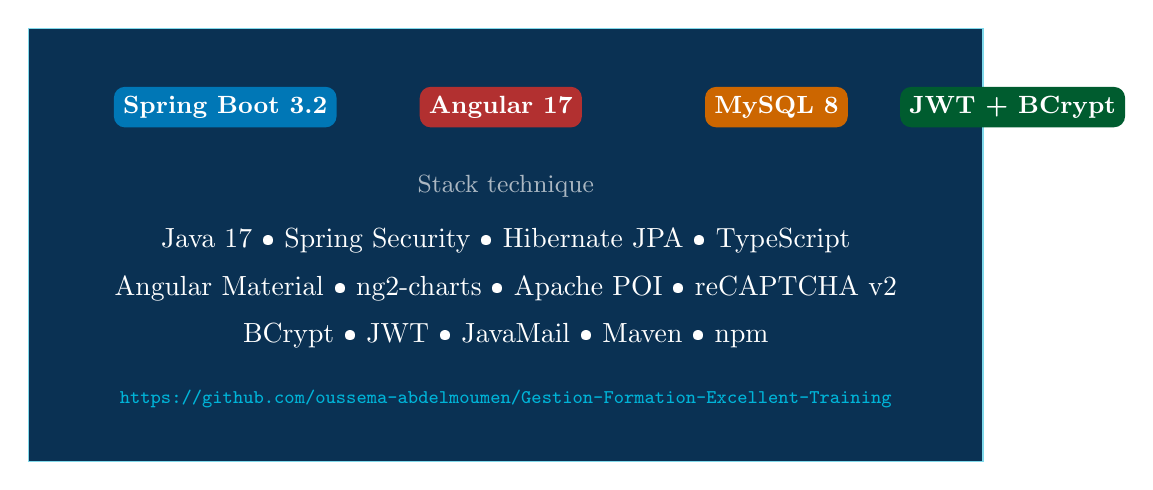
\begin{tikzpicture}
  \fill[medblue!20!darkblue] (0,0) rectangle (\textwidth, 5.5cm);
  \draw[lightblue!50, line width=0.5pt] (0,0) rectangle (\textwidth, 5.5cm);
  % Tech badges
  \node[fill=medblue, rounded corners=4pt, text=white, font=\bfseries\small] at (2.5,4.5) {Spring Boot 3.2};
  \node[fill=red!70!black, rounded corners=4pt, text=white, font=\bfseries\small] at (6,4.5) {Angular 17};
  \node[fill=orange!80!black, rounded corners=4pt, text=white, font=\bfseries\small] at (9.5,4.5) {MySQL 8};
  \node[fill=green!40!black, rounded corners=4pt, text=white, font=\bfseries\small] at (12.5,4.5) {JWT + BCrypt};
  % Stack
  \node[text=gray!70, font=\small] at (\textwidth/2, 3.5) {Stack technique};
  \node[text=white, font=\normalsize] at (\textwidth/2, 2.8) {Java 17 \textbullet\ Spring Security \textbullet\ Hibernate JPA \textbullet\ TypeScript};
  \node[text=white, font=\normalsize] at (\textwidth/2, 2.2) {Angular Material \textbullet\ ng2-charts \textbullet\ Apache POI \textbullet\ reCAPTCHA v2};
  \node[text=white, font=\normalsize] at (\textwidth/2, 1.6) {BCrypt \textbullet\ JWT \textbullet\ JavaMail \textbullet\ Maven \textbullet\ npm};
  % Repo
  \node[text=lightblue, font=\scriptsize\ttfamily] at (\textwidth/2, 0.8) {\url{https://github.com/oussema-abdelmoumen/Gestion-Formation-Excellent-Training}};
\end{tikzpicture}

\vspace{1.2cm}
{\large\color{gray} R\'{e}alis\'{e} par}\\[0.3cm]
{\Large\bfseries\color{white} Oussema Abdelmoumen \quad \& \quad Malek Nasri}

\vfill

\begin{tikzpicture}
  \fill[medblue!40!darkblue] (0,0) rectangle (\textwidth, 1cm);
  \node at (\textwidth/2, 0.5cm) {\large\color{white}\bfseries Ann\'{e}e Universitaire 2025/2026};
\end{tikzpicture}
\end{titlepage}
\pagecolor{white}\color{black}

% ??? TABLE DES MATI\`{E}RES ???????????????????????????????
\tableofcontents
\clearpage

% ??????????????????????????????????????????????????????
\chapter*{R\'{e}sum\'{e}}
\addcontentsline{toc}{chapter}{R\'{e}sum\'{e}}

Ce rapport pr\'{e}sente la conception et le d\'{e}veloppement d'une application web compl\`{e}te de gestion de formation r\'{e}alis\'{e}e pour le centre \textbf{\og ~Excellent Training~\fg{}} de la soci\'{e}t\'{e} \textbf{Green Building}, dans le cadre du mini-projet de l'ISI Tunis El Manar pour l'ann\'{e}e universitaire 2025/2026.

L'application a \'{e}t\'{e} d\'{e}velopp\'{e}e avec une architecture full-stack moderne :
\begin{itemize}
  \item \textbf{Backend :} Spring Boot 3.2 (Java 17) avec Spring Security, JWT, JPA/Hibernate, MySQL, Apache POI
  \item \textbf{Frontend :} Angular 17 avec TypeScript, Angular Material, ng2-charts (Chart.js)
  \item \textbf{S\'{e}curit\'{e} :} Authentification JWT, BCrypt, reCAPTCHA v2, v\'{e}rification email
\end{itemize}

\noindent Le projet impl\'{e}mente un syst\`{e}me RBAC (Role-Based Access Control) avec trois r\^{o}les : Administrateur, Responsable et Utilisateur, chacun ayant des permissions distinctes sur les ressources de l'application.

\noindent En plus des fonctionnalit\'{e}s CRUD de base, l'application offre :
\begin{itemize}
  \item \textbf{Import Excel :} Importation en masse de formations, participants et formateurs via fichiers \texttt{.xlsx}
  \item \textbf{Suppression en lot :} S\'{e}lection multiple avec checkboxes pour supprimer plusieurs enregistrements
  \item \textbf{Dashboard avanc\'{e} :} Trois onglets (Vue d'ensemble, Gouvernance \& Budget, Participants \& Formateurs) avec filtrage par ann\'{e}e, zoom interactif sur les courbes, top participants les plus actifs, et top formateurs
  \item \textbf{Recherche en temps r\'{e}el :} Filtrage instantan\'{e} sur tous les champs dans toutes les pages
\end{itemize}

\clearpage

% ??????????????????????????????????????????????????????
\chapter{Introduction G\'{e}n\'{e}rale}
% ??????????????????????????????????????????????????????

\section{Contexte et Probl\'{e}matique}

La formation professionnelle continue est un droit fondamental pour tout personnel d'une entreprise ou d'une administration. Elle permet \`{a} chaque individu d'acqu\'{e}rir de nouveaux savoirs et savoir-faire, am\'{e}liorant ainsi ses comp\'{e}tences par des techniques et connaissances actualis\'{e}es \cite{cdc2026}.

Le centre de formation \textbf{\og ~Excellent Training~\fg{}} de la soci\'{e}t\'{e} \textbf{Green Building} organisait jusqu'alors ses formations de mani\`{e}re enti\`{e}rement manuelle :

\begin{itemize}
  \item Les structures envoyaient leurs besoins en format \textbf{papier}
  \item Les informations \'{e}taient saisies dans des \textbf{fichiers Excel} cr\'{e}\'{e}s chaque ann\'{e}e
  \item Absence totale de suivi statistique et d'\'{e}valuation automatis\'{e}e
  \item Risques \'{e}lev\'{e}s d'erreurs humaines et de perte de donn\'{e}es
\end{itemize}

\begin{warnbox}{Probl\`{e}mes identifi\'{e}s}
  Perte de temps --- Erreurs de saisie --- Impossible de faire des statistiques par domaine ou structure --- Pas de tra\c{c}abilit\'{e} des cr\'{e}ateurs de formations --- Donn\'{e}es \'{e}parpill\'{e}es dans plusieurs fichiers Excel
\end{warnbox}

\section{Objectifs du Projet}

\begin{successbox}{Solution propos\'{e}e}
D\'{e}velopper une application web full-stack permettant de centraliser, s\'{e}curiser et automatiser la gestion des formations, avec un contr\^{o}le d'acc\`{e}s granulaire par r\^{o}les.
\end{successbox}

\begin{itemize}
  \item Centraliser toutes les donn\'{e}es en base de donn\'{e}es MySQL relationnelle
  \item Impl\'{e}menter un syst\`{e}me RBAC avec 3 niveaux d'acc\`{e}s distincts
  \item Fournir un tableau de bord statistique interactif avec filtrage par ann\'{e}e et zoom
  \item Assurer la s\'{e}curit\'{e} des donn\'{e}es (JWT, BCrypt, CAPTCHA, v\'{e}rification email)
  \item Offrir une interface moderne avec dark/light mode et contr\^{o}les de saisie rigoureux
  \item Permettre l'export et l'import des donn\'{e}es en fichier Excel (\texttt{.xlsx})
  \item Permettre la suppression en lot (multi-s\'{e}lection) de participants et formateurs
  \item Impl\'{e}menter une recherche en temps r\'{e}el sur tous les champs
\end{itemize}

\section{P\'{e}rim\`{e}tre fonctionnel}

Le projet couvre les cas d'utilisation du cahier des charges \cite{cdc2026} :

\begin{table}[H]
\centering
\caption{Cas d'utilisation principaux}
\begin{tabularx}{\textwidth}{|L{3.5cm}|X|}
\hline
\rowcolor{darkblue} \textcolor{white}{\textbf{Cas d'utilisation}} & \textcolor{cyan}{\textbf{Description}} \\
\hline
Gestion des formations & CRUD complet + organisation (formateur, participants, lieu, date) \\
\hline
Gestion des participants & CRUD avec affiliation structure/profil et vue des formations associ\'{e}es \\
\hline
Gestion des formateurs & CRUD avec distinction interne/externe \\
\hline
Statistiques & Dashboard 3 onglets avec graphiques interactifs, filtrage par ann\'{e}e et zoom \\
\hline
Authentification & Login, inscription, v\'{e}rification email, CAPTCHA \\
\hline
Export Excel & Fichier .xlsx avec mise en forme pour formations \\
\hline
Import Excel & Import en masse de formations, participants et formateurs via .xlsx \\
\hline
Suppression en lot & Multi-s\'{e}lection avec checkboxes pour supprimer plusieurs enregistrements \\
\hline
Recherche temps r\'{e}el & Filtrage instantan\'{e} sur tous les champs dans toutes les pages \\
\hline
Gestion utilisateurs & CRUD comptes (Admin uniquement) \\
\hline
\end{tabularx}
\end{table}

\clearpage

% ??????????????????????????????????????????????????????
\chapter{Architecture et Conception}
% ??????????????????????????????????????????????????????

\section{Architecture G\'{e}n\'{e}rale}

L'application suit une architecture \textbf{Client-Serveur \`{a} trois couches} (\textit{3-tier archi\-tecture}), communiquant via une \textbf{API REST} s\'{e}curis\'{e}e par JWT :

\begin{figure}[H]
\centering
\resizebox{\textwidth}{!}{%
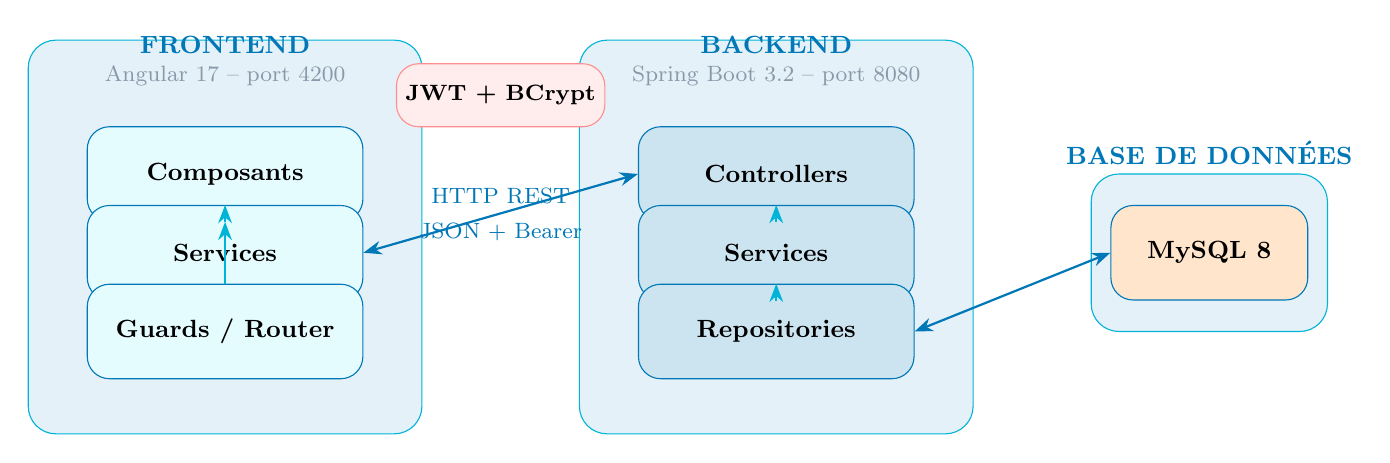
\begin{tikzpicture}[
  box/.style={draw=medblue, fill=lightbg, rounded corners=8pt, minimum width=3.5cm, minimum height=1.2cm, text centered, font=\small\bfseries},
  layerbox/.style={draw=lightblue, fill=medblue!10, rounded corners=10pt, inner sep=10pt},
  arrow/.style={-Stealth, thick, color=lightblue},
  darrow/.style={Stealth-Stealth, thick, color=medblue}
]
  % Frontend Layer
  \node[layerbox, minimum width=5cm, minimum height=5cm] (fe) at (0,0) {};
  \node[above] at (0, 2.2) {\color{medblue}\bfseries\small FRONTEND};
  \node[above] at (0, 1.8) {\color{gray}\footnotesize Angular 17 -- port 4200};
  \node[box, fill=cyan!10] (comp) at (0, 0.8) {Composants};
  \node[box, fill=cyan!10] (srv) at (0, -0.2) {Services};
  \node[box, fill=cyan!10] (guard) at (0, -1.2) {Guards / Router};

  % Backend Layer
  \node[layerbox, minimum width=5cm, minimum height=5cm] (be) at (7,0) {};
  \node[above] at (7, 2.2) {\color{medblue}\bfseries\small BACKEND};
  \node[above] at (7, 1.8) {\color{gray}\footnotesize Spring Boot 3.2 -- port 8080};
  \node[box, fill=medblue!20] (ctrl) at (7, 0.8) {Controllers};
  \node[box, fill=medblue!20] (bsrv) at (7, -0.2) {Services};
  \node[box, fill=medblue!20] (repo) at (7, -1.2) {Repositories};

  % DB Layer
  \node[layerbox, minimum width=3cm, minimum height=2cm] (db) at (12.5, -0.2) {};
  \node[box, fill=orange!20, minimum width=2.5cm] (mysql) at (12.5, -0.2) {MySQL 8};
  \node[above] at (12.5, 0.8) {\color{medblue}\bfseries\small BASE DE DONN\'{E}ES};

  % Security
  \node[box, fill=red!10, draw=red!60, minimum width=2.5cm, minimum height=0.8cm] (jwt) at (3.5, 1.8) {\footnotesize JWT + BCrypt};

  % Arrows
  \draw[darrow] (srv.east) -- node[above, font=\footnotesize] {HTTP REST} node[below, font=\footnotesize\color{gray}] {JSON + Bearer} (ctrl.west);
  \draw[arrow] (ctrl.south) -- (bsrv.north);
  \draw[arrow] (bsrv.south) -- (repo.north);
  \draw[darrow] (repo.east) -- (mysql.west);
  \draw[arrow] (comp.south) -- (srv.north);
  \draw[arrow] (guard.north) -- (comp.south);
\end{tikzpicture}%
}
\caption{Architecture 3-tiers de l'application}
\label{fig:archi}
\end{figure}

\section{Structure du Backend (Spring Boot)}

Le backend est organis\'{e} en \textbf{4 couches} selon le patron d'architecture MVC :

\begin{figure}[H]
\centering
\resizebox{0.88\textwidth}{!}{%
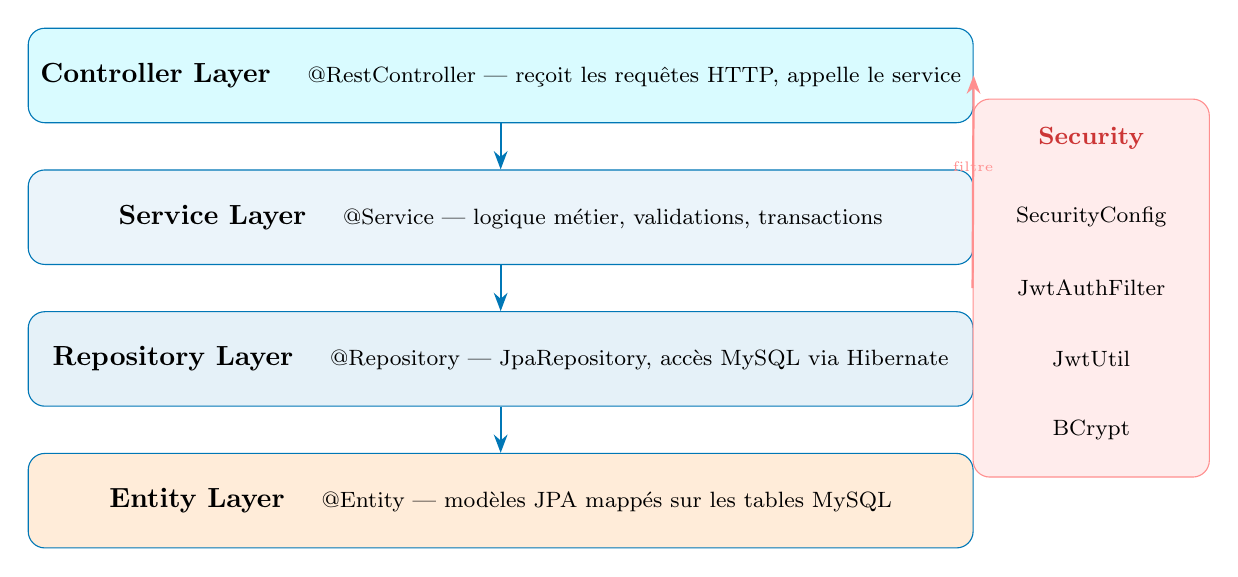
\begin{tikzpicture}[
  layer/.style={draw=medblue, fill=#1, rounded corners=6pt, minimum width=12cm, minimum height=1.2cm, text centered},
  arrow/.style={-Stealth, thick, color=medblue}
]
  \node[layer=cyan!15] (ctrl) at (0,0) {\textbf{Controller Layer} \quad \footnotesize @RestController --- re\c{c}oit les requ\^{e}tes HTTP, appelle le service};
  \node[layer=lightbg] (svc) at (0,-1.8) {\textbf{Service Layer} \quad \footnotesize @Service --- logique m\'{e}tier, validations, transactions};
  \node[layer=medblue!10] (rep) at (0,-3.6) {\textbf{Repository Layer} \quad \footnotesize @Repository --- JpaRepository, acc\`{e}s MySQL via Hibernate};
  \node[layer=orange!15] (ent) at (0,-5.4) {\textbf{Entity Layer} \quad \footnotesize @Entity --- mod\`{e}les JPA mapp\'{e}s sur les tables MySQL};
  % Security on the side
  \node[draw=red!60, fill=red!10, rounded corners=6pt, minimum width=3cm, minimum height=4.8cm] (sec) at (7.5,-2.7) {};
  \node[text=red!80!black, font=\bfseries\small] at (7.5,-0.8) {Security};
  \node[font=\footnotesize, align=center] at (7.5,-1.8) {SecurityConfig};
  \node[font=\footnotesize, align=center] at (7.5,-2.7) {JwtAuthFilter};
  \node[font=\footnotesize, align=center] at (7.5,-3.6) {JwtUtil};
  \node[font=\footnotesize, align=center] at (7.5,-4.5) {BCrypt};

  \draw[arrow] (ctrl.south) -- (svc.north);
  \draw[arrow] (svc.south) -- (rep.north);
  \draw[arrow] (rep.south) -- (ent.north);
  \draw[-Stealth, red!60, thick] (sec.west) -- (ctrl.east) node[midway, above, font=\tiny] {filtre};
\end{tikzpicture}%
}
\caption{Architecture en couches du backend Spring Boot}
\label{fig:backend}
\end{figure}

\section{Structure du Frontend (Angular)}

\begin{table}[H]
\centering
\caption{Organisation des modules Angular}
\small
\begin{tabularx}{\textwidth}{|L{4.2cm}|X|}
\hline
\rowcolor{darkblue} \textcolor{white}{\textbf{Dossier}} & \textcolor{cyan}{\textbf{Contenu et r\^{o}le}} \\
\hline
\texttt{core/services/} & AuthService, FormationService, ParticipantService, FormateurService, ThemeService --- communication API \\
\hline
\texttt{core/guards/} & AuthGuard (connexion requise), RoleGuard (v\'{e}rification du r\^{o}le) \\
\hline
\texttt{core/interceptors/} & JwtInterceptor --- ajout automatique du Bearer token \\
\hline
\texttt{features/auth/} & Login, Register, VerifyEmail \\
\hline
\texttt{features/landing/} & Page d'accueil publique anim\'{e}e \\
\hline
\texttt{features/dashboard/} & Tableau de bord 3 onglets avec zoom, filtrage ann\'{e}e et stats dynamiques \\
\hline
\texttt{features/formations/} & CRUD formations + export/import Excel + recherche temps r\'{e}el \\
\hline
\texttt{features/participants/} & CRUD + import Excel + suppression en lot + panel formations \\
\hline
\texttt{features/formateurs/} & CRUD + import Excel + suppression en lot \\
\hline
\texttt{shared/models/} & Interfaces TypeScript (Formation, Participant, Formateur\ldots) \\
\hline
\end{tabularx}
\end{table}

\clearpage
% ??????????????????????????????????????????????????????
\chapter{Mod\`{e}le de Donn\'{e}es}
% ??????????????????????????????????????????????????????

\section{Diagramme Entit\'{e}-Association}

\begin{figure}[H]
\centering
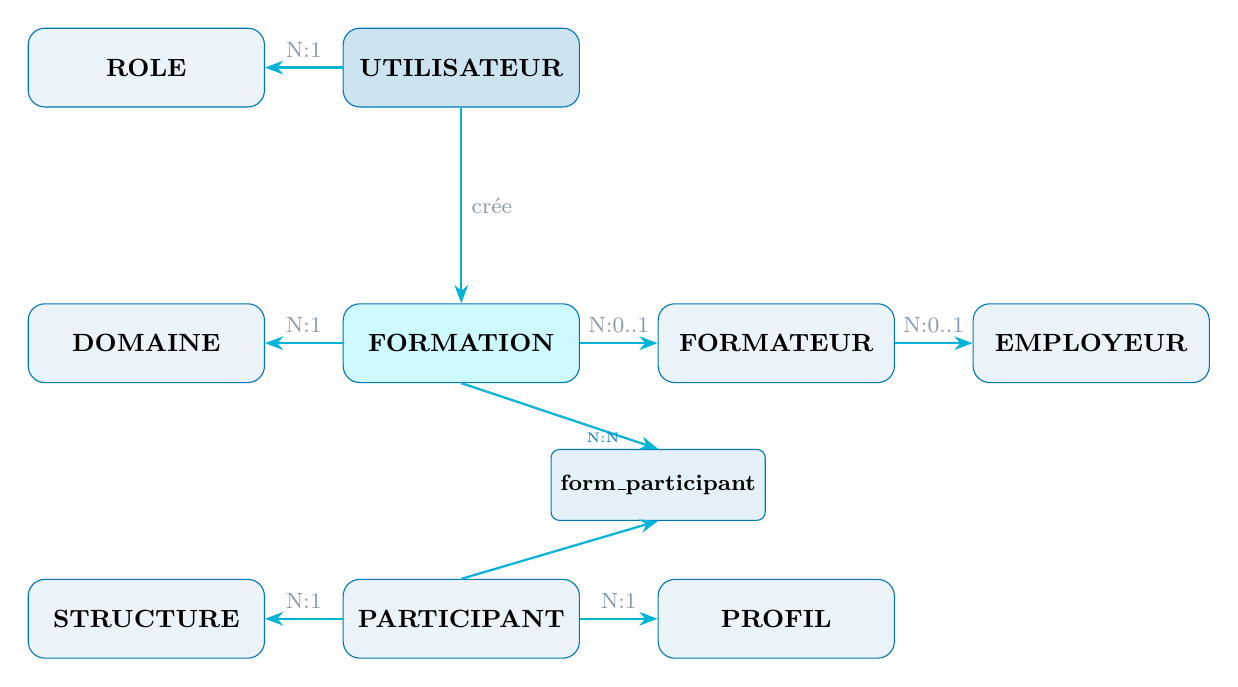
\begin{tikzpicture}[
  entity/.style={draw=medblue, fill=lightbg, rounded corners=6pt, minimum width=3cm, minimum height=1cm, text centered, font=\small\bfseries},
  relation/.style={draw=lightblue, -Stealth, thick},
  label/.style={font=\footnotesize\color{gray}, midway}
]
  % Entities
  \node[entity, fill=cyan!20] (form) at (4, 0) {FORMATION};
  \node[entity] (dom) at (0, 0) {DOMAINE};
  \node[entity] (fmt) at (8, 0) {FORMATEUR};
  \node[entity] (emp) at (12, 0) {EMPLOYEUR};
  \node[entity] (part) at (4, -3.5) {PARTICIPANT};
  \node[entity] (str) at (0, -3.5) {STRUCTURE};
  \node[entity] (prof) at (8, -3.5) {PROFIL};
  \node[entity, fill=medblue!20] (util) at (4, 3.5) {UTILISATEUR};
  \node[entity] (role) at (0, 3.5) {ROLE};
  \node[entity, fill=medblue!10, rounded corners=3pt, minimum width=2.2cm, minimum height=0.9cm, font=\footnotesize\bfseries] (fp) at (6.5, -1.8) {form\_participant};

  % Relations
  \draw[relation] (form.west) -- node[label, above] {N:1} (dom.east);
  \draw[relation] (form.east) -- node[label, above] {N:0..1} (fmt.west);
  \draw[relation] (fmt.east) -- node[label, above] {N:0..1} (emp.west);
  \draw[relation] (form.south) -- (fp.north);
  \draw[relation] (part.north) -- (fp.south);
  \draw[relation] (part.west) -- node[label, above] {N:1} (str.east);
  \draw[relation] (part.east) -- node[label, above] {N:1} (prof.west);
  \draw[relation] (util.south) -- node[label, right] {cr\'{e}e} (form.north);
  \draw[relation] (util.west) -- node[label, above] {N:1} (role.east);

  % Labels on relation tables
  \node[font=\tiny\color{medblue}] at (5.8, -1.2) {N:N};
\end{tikzpicture}
\caption{Diagramme Entit\'{e}-Association simplifi\'{e}}
\label{fig:er}
\end{figure}

\section{Description des Tables}

\begin{table}[H]
\centering
\caption{Tables principales de la base \texttt{gestion\_formation}}
\footnotesize
\begin{tabularx}{\textwidth}{|L{4cm}|X|L{3.5cm}|}
\hline
\rowcolor{darkblue} \textcolor{white}{\textbf{Table}} & \textcolor{cyan}{\textbf{Attributs principaux}} & \textcolor{white}{\textbf{Remarques}} \\
\hline
\texttt{role} & id (PK), nom & 3 valeurs : ADMIN, RESPONSABLE, UTILISATEUR \\
\hline
\texttt{utilisateur} & id, login (UK), password, email (UK), id\_role (FK), email\_verifie, actif, token\_verification & V\'{e}rification email avant activation \\
\hline
\texttt{formation} & id, titre, annee, duree, budget, lieu, date\_formation, id\_domaine (FK), id\_formateur (FK), created\_by\_id & Entit\'{e} centrale du syst\`{e}me \\
\hline
\texttt{formation\_participant} & id\_formation, id\_participant & Table d'association N-N \\
\hline
\texttt{participant} & id, nom, prenom, email, tel, id\_structure (FK), id\_profil (FK) & Li\'{e} \`{a} structure et profil \\
\hline
\texttt{formateur} & id, nom, prenom, email, tel, type (INTERNE/EXTERNE), id\_employeur (FK) & Distinction interne/externe \\
\hline
\texttt{domaine} & id, libelle (UK) & Ex: Informatique, Finance \\
\hline
\texttt{structure} & id, libelle (UK) & Direction centrale/r\'{e}gionale \\
\hline
\texttt{profil} & id, libelle (UK) & Ex: Informaticien Bac+5 \\
\hline
\texttt{employeur} & id, nom\_employeur (UK) & Pour formateurs externes \\
\hline
\end{tabularx}
\normalsize
\end{table}

\section{Script SQL de cr\'{e}ation}

\begin{lstlisting}[style=sqlstyle, caption={Extrait du script schema.sql}]
CREATE DATABASE IF NOT EXISTS gestion_formation
  CHARACTER SET utf8mb4 COLLATE utf8mb4_unicode_ci;
USE gestion_formation;

CREATE TABLE role (
  id  INT PRIMARY KEY AUTO_INCREMENT,
  nom VARCHAR(50) NOT NULL UNIQUE
);
INSERT INTO role(nom) VALUES ('ADMIN'),('RESPONSABLE'),('UTILISATEUR');

CREATE TABLE utilisateur (
  id                   INT PRIMARY KEY AUTO_INCREMENT,
  login                VARCHAR(100) NOT NULL UNIQUE,
  password             VARCHAR(255) NOT NULL,
  email                VARCHAR(150) UNIQUE,
  id_role              INT NOT NULL,
  email_verifie        BOOLEAN DEFAULT FALSE,
  actif                BOOLEAN DEFAULT FALSE,
  token_verification   VARCHAR(100),
  FOREIGN KEY (id_role) REFERENCES role(id)
);

CREATE TABLE formation (
  id              BIGINT PRIMARY KEY AUTO_INCREMENT,
  titre           VARCHAR(200) NOT NULL,
  annee           INT,  duree INT,  budget DOUBLE,
  lieu            VARCHAR(200),
  date_formation  DATE,
  id_domaine      INT,
  id_formateur    INT,
  created_by_id   INT,
  FOREIGN KEY (id_domaine)  REFERENCES domaine(id),
  FOREIGN KEY (id_formateur) REFERENCES formateur(id)
);

-- Relation N-N
CREATE TABLE formation_participant (
  id_formation   BIGINT, id_participant INT,
  PRIMARY KEY (id_formation, id_participant)
);
\end{lstlisting}

\clearpage
% ??????????????????????????????????????????????????????
\chapter{S\'{e}curit\'{e} et Authentification}
% ??????????????????????????????????????????????????????

\section{Flux d'Authentification JWT}

\begin{figure}[H]
\centering
\resizebox{\textwidth}{!}{%
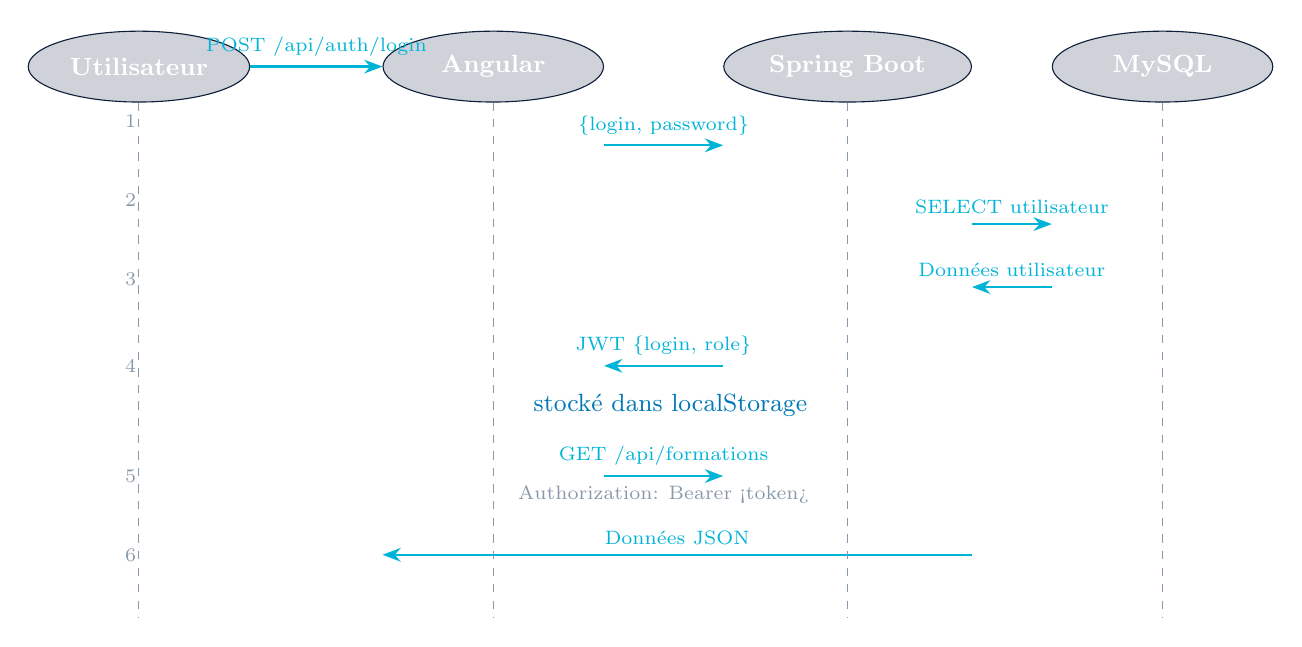
\begin{tikzpicture}[
  node distance=0.9cm,
  step/.style={draw=medblue, fill=lightbg, rounded corners=5pt, minimum width=3.5cm, minimum height=0.8cm, text centered, font=\small},
  arrow/.style={-Stealth, thick, color=lightblue},
  actor/.style={draw=darkblue, fill=darkblue!20, ellipse, minimum width=2.8cm, minimum height=0.9cm, text=white, font=\bfseries\small}
]
  \node[actor] (user) at (0,0) {Utilisateur};
  \node[actor] (fe)   at (4.5,0) {Angular};
  \node[actor] (be)   at (9,0) {Spring Boot};
  \node[actor] (db)   at (13,0) {MySQL};

  % Step 1
  \draw[arrow] (user.east) -- node[above,font=\scriptsize]{POST /api/auth/login} (fe.west);
  % Step 2
  \draw[arrow] ([yshift=-1cm]fe.east) -- node[above,font=\scriptsize]{\{login, password\}} ([yshift=-1cm]be.west);
  % Step 3
  \draw[arrow] ([yshift=-2cm]be.east) -- node[above,font=\scriptsize]{SELECT utilisateur} ([yshift=-2cm]db.west);
  \draw[arrow] ([yshift=-2.8cm]db.west) -- node[above,font=\scriptsize]{Donn\'{e}es utilisateur} ([yshift=-2.8cm]be.east);
  % Step 4
  \draw[arrow] ([yshift=-3.8cm]be.west) -- node[above,font=\scriptsize]{JWT \{login, role\}} ([yshift=-3.8cm]fe.east);
  \node[font=\small, color=medblue] at (6.75,-4.3) {stock\'{e} dans localStorage};
  % Step 5
  \draw[arrow] ([yshift=-5.2cm]fe.east) -- node[above,font=\scriptsize]{GET /api/formations} node[below,font=\scriptsize,color=gray]{Authorization: Bearer <token>} ([yshift=-5.2cm]be.west);
  % Step 6
  \draw[arrow] ([yshift=-6.2cm]be.east) -- node[above,font=\scriptsize]{Donn\'{e}es JSON} ([yshift=-6.2cm]fe.west);

  % Vertical lines
  \draw[dashed, gray] (user.south) -- (0,-7);
  \draw[dashed, gray] (fe.south)   -- (4.5,-7);
  \draw[dashed, gray] (be.south)   -- (9,-7);
  \draw[dashed, gray] (db.south)   -- (13,-7);

  % Step labels
  \node[font=\scriptsize, color=gray, right] at (-0.3,-0.7) {1};
  \node[font=\scriptsize, color=gray, right] at (-0.3,-1.7) {2};
  \node[font=\scriptsize, color=gray, right] at (-0.3,-2.7) {3};
  \node[font=\scriptsize, color=gray, right] at (-0.3,-3.8) {4};
  \node[font=\scriptsize, color=gray, right] at (-0.3,-5.2) {5};
  \node[font=\scriptsize, color=gray, right] at (-0.3,-6.2) {6};
\end{tikzpicture}%
}
\caption{Diagramme de s\'{e}quence --- Authentification JWT}
\label{fig:jwt}
\end{figure}

\section{Impl\'{e}mentation JWT}

\begin{lstlisting}[language=Java, caption={JwtUtil.java --- G\'{e}n\'{e}ration et validation du token}]
@Component
public class JwtUtil {

    @Value("${jwt.secret}")
    private String secret;

    // G\'{e}n\'{e}ration du token avec le login ET le r\^{o}le
    public String generateToken(String username, String role) {
        return Jwts.builder()
            .setSubject(username)
            .claim("role", role)       // R\^{o}le inclus dans le token
            .setIssuedAt(new Date())
            .setExpiration(new Date(System.currentTimeMillis() + 86400000L))
            .signWith(getSigningKey(), SignatureAlgorithm.HS256)
            .compact();
    }

    // Extraction du r\^{o}le depuis le token
    public String extractRole(String token) {
        return (String) getClaims(token).get("role");
    }

    public boolean isTokenValid(String token) {
        try { getClaims(token); return true; }
        catch (JwtException e) { return false; }
    }
}
\end{lstlisting}

\section{Configuration Spring Security}

\begin{lstlisting}[language=Java, caption={SecurityConfig.java --- R\`{e}gles d'acc\`{e}s par endpoint}]
@EnableMethodSecurity(prePostEnabled = true)
public class SecurityConfig {

  @Bean
  public SecurityFilterChain filterChain(HttpSecurity http) throws Exception {
    http
      .authorizeHttpRequests(auth -> auth
        // Public : login, register, v\'{e}rification email
        .requestMatchers("/api/auth/**").permitAll()

        // Lecture pour tous les r\^{o}les (pour remplir les formulaires)
        .requestMatchers(HttpMethod.GET, "/api/domaines/**").authenticated()
        .requestMatchers(HttpMethod.GET, "/api/structures/**").authenticated()

        // \'{E}criture r\'{e}serv\'{e}e \`{a} ADMIN uniquement
        .requestMatchers("/api/utilisateurs/**").hasRole("ADMIN")
        .requestMatchers(HttpMethod.POST, "/api/domaines/**").hasRole("ADMIN")

        // RESPONSABLE + ADMIN peuvent g\'{e}rer les formations
        .requestMatchers(HttpMethod.POST, "/api/formations/**")
             .hasAnyRole("ADMIN","RESPONSABLE")

        // Tout le reste : \^{e}tre connect\'{e} suffit
        .anyRequest().authenticated()
      )
      .sessionManagement(s -> s.sessionCreationPolicy(STATELESS))
      .addFilterBefore(jwtAuthFilter, UsernamePasswordAuthenticationFilter.class);
    return http.build();
  }
}
\end{lstlisting}

\section{Inscription et V\'{e}rification Email}

Le processus d'inscription en auto-service est prot\'{e}g\'{e} par plusieurs m\'{e}canismes :

\begin{figure}[H]
\centering
\resizebox{0.62\textwidth}{!}{%
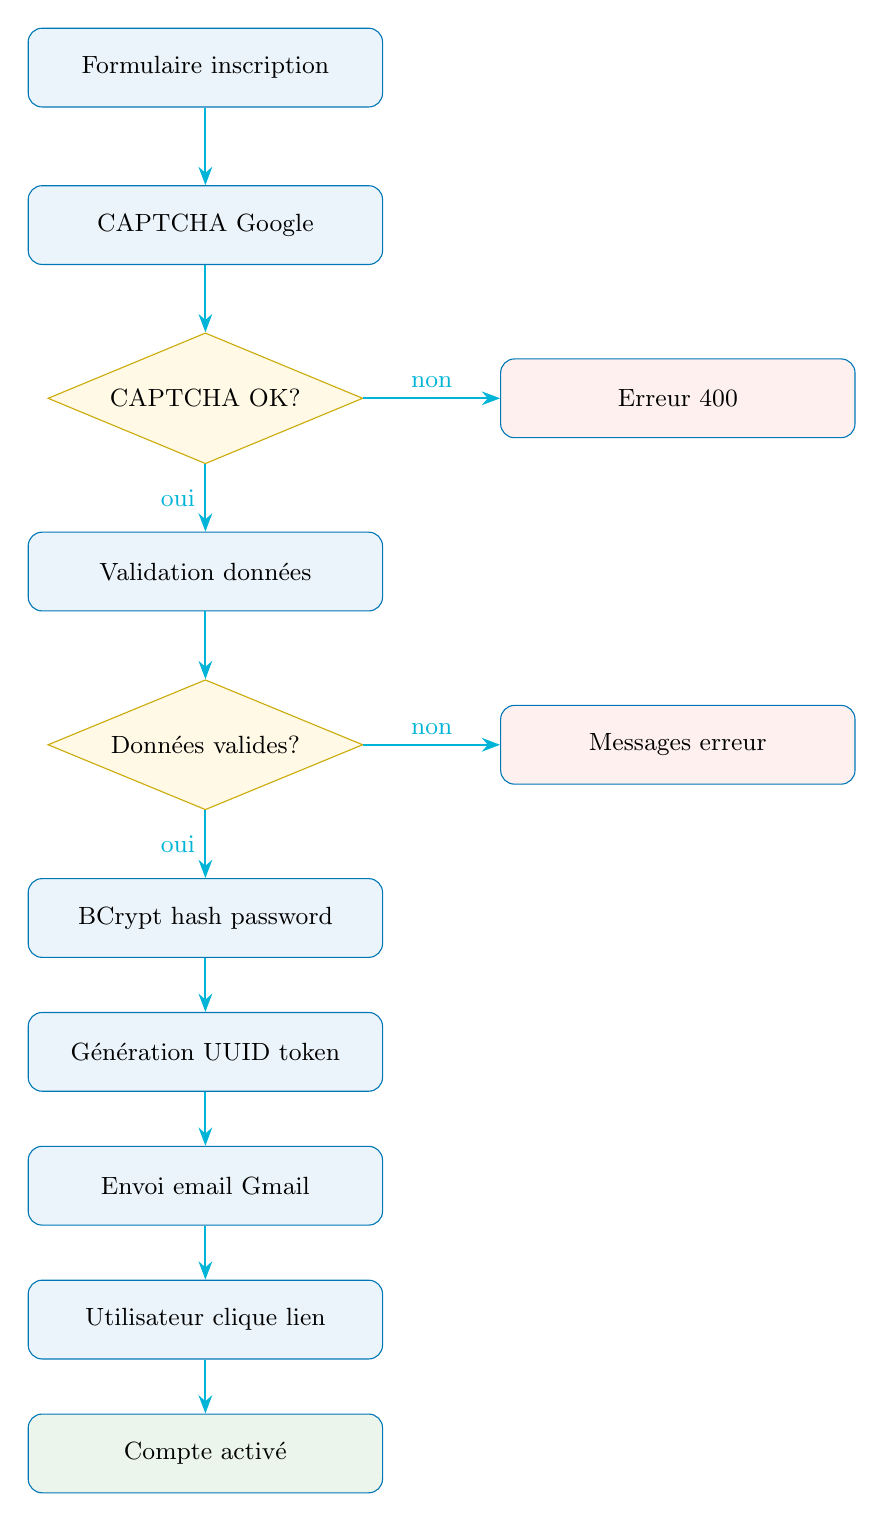
\begin{tikzpicture}[
  box/.style={draw=medblue, fill=lightbg, rounded corners=5pt, minimum width=4.5cm, minimum height=1cm, text centered, font=\small},
  arrow/.style={-Stealth, thick, color=lightblue},
  decision/.style={draw=gold!80!black, fill=lightyellow, diamond, aspect=2.2, minimum width=4cm, minimum height=1.2cm, text centered, font=\small}
]
  \node[box] (form)    at (0,0)     {Formulaire inscription};
  \node[box] (captcha) at (0,-2)    {CAPTCHA Google};
  \node[decision] (dca) at (0,-4.2) {CAPTCHA OK?};
  \node[box] (valid)   at (0,-6.4)  {Validation donn\'{e}es};
  \node[decision] (dv) at (0,-8.6)  {Donn\'{e}es valides?};
  \node[box] (hash)    at (0,-10.8) {BCrypt hash password};
  \node[box] (token)   at (0,-12.5) {G\'{e}n\'{e}ration UUID token};
  \node[box] (email)   at (0,-14.2) {Envoi email Gmail};
  \node[box] (click)   at (0,-15.9) {Utilisateur clique lien};
  \node[box, fill=lightgreen] (actif) at (0,-17.6) {Compte activ\'{e} \checkmark};
  % Errors (far enough right to avoid overlap)
  \node[box, fill=lightred] (ecap) at (6,-4.2) {Erreur 400};
  \node[box, fill=lightred] (eval) at (6,-8.6) {Messages erreur};

  \draw[arrow] (form)--(captcha);
  \draw[arrow] (captcha)--(dca);
  \draw[arrow] (dca)--node[left,font=\small]{oui}(valid);
  \draw[arrow] (dca)--node[above,font=\small]{non}(ecap);
  \draw[arrow] (valid)--(dv);
  \draw[arrow] (dv)--node[left,font=\small]{oui}(hash);
  \draw[arrow] (dv)--node[above,font=\small]{non}(eval);
  \draw[arrow] (hash)--(token);
  \draw[arrow] (token)--(email);
  \draw[arrow] (email)--(click);
  \draw[arrow] (click)--(actif);
\end{tikzpicture}%
}
\caption{Flux d'inscription avec v\'{e}rification email}
\label{fig:register}
\end{figure}

\begin{infobox}{R\`{e}gles du mot de passe fort (inscription uniquement)}
  Minimum 8 caract\`{e}res \textbullet{} Au moins 1 majuscule \textbullet{} Au moins 1 minuscule \textbullet{} Au moins 1 chiffre \textbullet{} Au moins 1 caract\`{e}re sp\'{e}cial (\texttt{!@\#\$\%\^{}\&*...})
\end{infobox}

\clearpage
% ??????????????????????????????????????????????????????
\chapter{Gestion des R\^{o}les (RBAC)}
% ??????????????????????????????????????????????????????

\section{Les Trois R\^{o}les}

\begin{figure}[H]
\centering
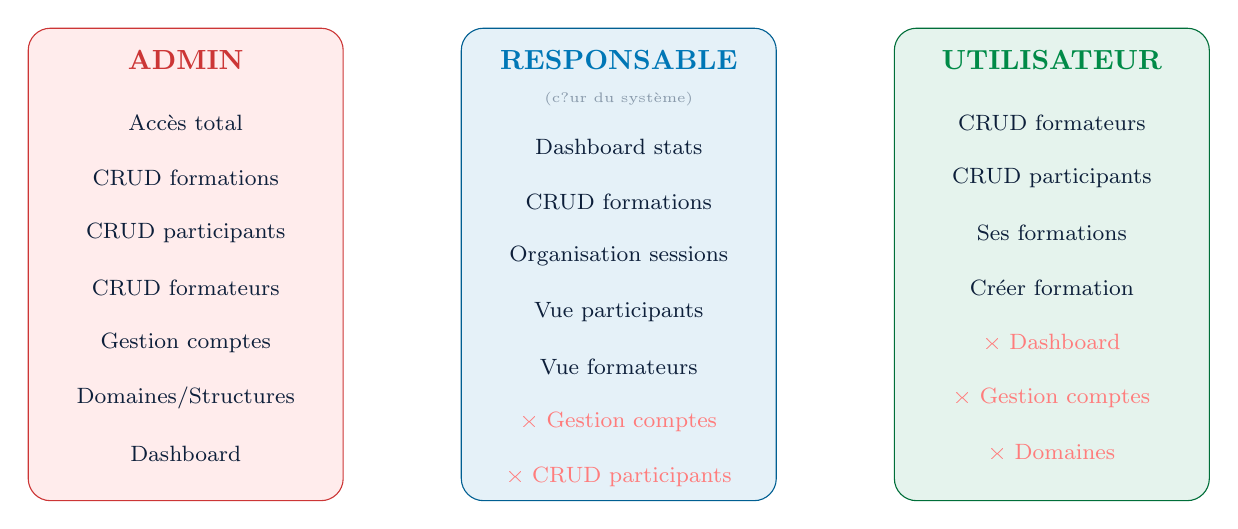
\begin{tikzpicture}[
  role/.style={draw=#1!80!black, fill=#1!10, rounded corners=8pt, minimum width=4cm, minimum height=6cm},
  item/.style={font=\footnotesize, text=darkblue}
]
  % ADMIN
  \node[role=red] (admin) at (0,0) {};
  \node[font=\bfseries\color{red!80!black}] at (0, 2.6) {ADMIN};
  \node[item] at (0, 1.8) {\checkmark Acc\`{e}s total};
  \node[item] at (0, 1.1) {\checkmark CRUD formations};
  \node[item] at (0, 0.4) {\checkmark CRUD participants};
  \node[item] at (0,-0.3) {\checkmark CRUD formateurs};
  \node[item] at (0,-1.0) {\checkmark Gestion comptes};
  \node[item] at (0,-1.7) {\checkmark Domaines/Structures};
  \node[item] at (0,-2.4) {\checkmark Dashboard};

  % RESPONSABLE
  \node[role=medblue] (resp) at (5.5,0) {};
  \node[font=\bfseries\color{medblue}] at (5.5, 2.6) {RESPONSABLE};
  \node[font=\tiny\color{gray}] at (5.5, 2.1) {(c?ur du syst\`{e}me)};
  \node[item] at (5.5, 1.5) {\checkmark Dashboard stats};
  \node[item] at (5.5, 0.8) {\checkmark CRUD formations};
  \node[item] at (5.5, 0.1) {\checkmark Organisation sessions};
  \node[item] at (5.5,-0.6) {\checkmark Vue participants};
  \node[item] at (5.5,-1.3) {\checkmark Vue formateurs};
  \node[item, text=red!70] at (5.5,-2.0) {\texttimes{} Gestion comptes};
  \node[item, text=red!70] at (5.5,-2.7) {\texttimes{} CRUD participants};

  % UTILISATEUR
  \node[role=green!60!black] (user) at (11,0) {};
  \node[font=\bfseries\color{green!60!black}] at (11, 2.6) {UTILISATEUR};
  \node[item] at (11, 1.8) {\checkmark CRUD formateurs};
  \node[item] at (11, 1.1) {\checkmark CRUD participants};
  \node[item] at (11, 0.4) {\checkmark Ses formations};
  \node[item] at (11,-0.3) {\checkmark Cr\'{e}er formation};
  \node[item, text=red!70] at (11,-1.0) {\texttimes{} Dashboard};
  \node[item, text=red!70] at (11,-1.7) {\texttimes{} Gestion comptes};
  \node[item, text=red!70] at (11,-2.4) {\texttimes{} Domaines};
\end{tikzpicture}
\caption{Permissions par r\^{o}le}
\label{fig:roles}
\end{figure}

\section{Tableau des Permissions D\'{e}taill\'{e}es}

\begin{table}[H]
\centering
\caption{Matrice des permissions RBAC}
\small
\begin{tabularx}{\textwidth}{|X|C{2.2cm}|C{2.8cm}|C{2.8cm}|}
\hline
\rowcolor{darkblue}
\textcolor{white}{\textbf{Fonctionnalit\'{e}}} &
\textcolor{cyan}{\textbf{ADMIN}} &
\textcolor{cyan}{\textbf{RESPONSABLE}} &
\textcolor{cyan}{\textbf{UTILISATEUR}} \\
\hline
Dashboard / statistiques & \textcolor{green!50!black}{\checkmark} & \textcolor{green!50!black}{\checkmark} & \textcolor{red}{\texttimes} \\
\hline
Voir formations & \textcolor{green!50!black}{\checkmark} & \textcolor{green!50!black}{\checkmark} & \textcolor{green!50!black}{\checkmark} \\
\hline
CRUD formations & \textcolor{green!50!black}{\checkmark} & \textcolor{green!50!black}{\checkmark} & \textcolor{orange!80!black}{Ses propres} \\
\hline
Organisation formation & \textcolor{green!50!black}{\checkmark} & \textcolor{green!50!black}{\checkmark} & \textcolor{red}{\texttimes} \\
\hline
CRUD participants & \textcolor{green!50!black}{\checkmark} & \textcolor{red}{\texttimes} & \textcolor{green!50!black}{\checkmark} \\
\hline
CRUD formateurs & \textcolor{green!50!black}{\checkmark} & \textcolor{red}{\texttimes} & \textcolor{green!50!black}{\checkmark} \\
\hline
Export Excel & \textcolor{green!50!black}{\checkmark} & \textcolor{green!50!black}{\checkmark} & \textcolor{red}{\texttimes} \\
\hline
Import Excel & \textcolor{green!50!black}{\checkmark} & \textcolor{green!50!black}{\checkmark} & \textcolor{red}{\texttimes} \\
\hline
Suppression en lot & \textcolor{green!50!black}{\checkmark} & \textcolor{red}{\texttimes} & \textcolor{green!50!black}{\checkmark} \\
\hline
Domaines (lecture) & \textcolor{green!50!black}{\checkmark} & \textcolor{green!50!black}{\checkmark} & \textcolor{green!50!black}{\checkmark} \\
\hline
Domaines (\'{e}criture) & \textcolor{green!50!black}{\checkmark} & \textcolor{red}{\texttimes} & \textcolor{red}{\texttimes} \\
\hline
Gestion utilisateurs & \textcolor{green!50!black}{\checkmark} & \textcolor{red}{\texttimes} & \textcolor{red}{\texttimes} \\
\hline
\end{tabularx}
\end{table}

\section{Guards Angular}

\begin{lstlisting}[language=Java, caption={RoleGuard --- Protection des routes par r\^{o}le}]
@Injectable({ providedIn: 'root' })
export class RoleGuard implements CanActivate {

  canActivate(route: ActivatedRouteSnapshot): boolean {
    // R\'{e}cup\`{e}re les r\^{o}les autoris\'{e}s depuis la configuration de la route
    const allowedRoles: string[] = route.data['roles'] || [];
    const userRole = this.auth.getRole(); // Depuis localStorage

    if (allowedRoles.length === 0 || allowedRoles.includes(userRole!))
      return true;

    // Acc\`{e}s refus\'{e} ? page 403
    this.router.navigate(['/access-denied']);
    return false;
  }
}

// Utilisation dans le routing :
{ path: 'dashboard',
  component: DashboardComponent,
  canActivate: [RoleGuard],
  data: { roles: ['ADMIN', 'RESPONSABLE'] } // UTILISATEUR exclu
}
\end{lstlisting}

\clearpage
% ??????????????????????????????????????????????????????
\chapter{Impl\'{e}mentation Technique}
% ??????????????????????????????????????????????????????

\section{Entit\'{e}s JPA}

\begin{lstlisting}[language=Java, caption={Formation.java --- Entit\'{e} principale avec validation}]
@Entity
@Table(name = "formation")
@Data                    // Lombok : g\'{e}n\`{e}re getters/setters
@NoArgsConstructor       // Lombok : constructeur vide requis par JPA
public class Formation {

    @Id
    @GeneratedValue(strategy = GenerationType.IDENTITY)
    private Long id;

    @NotBlank(message = "Le titre est obligatoire")
    @Size(min = 3, max = 200, message = "3 \`{a} 200 caract\`{e}res")
    @Column(nullable = false, length = 200)
    private String titre;

    @NotNull(message = "L'ann\'{e}e est obligatoire")
    @Min(value = 2000)
    @Max(value = 2100)
    private Integer annee;

    @NotNull(message = "La dur\'{e}e est obligatoire")
    @Min(value = 1, message = "Minimum 1 jour")
    @Max(value = 365)
    private Integer duree;

    @DecimalMin(value = "0.0", message = "Budget non n\'{e}gatif")
    private Double budget;

    // Relations JPA (cl\'{e}s \'{e}trang\`{e}res)
    @NotNull(message = "Le domaine est obligatoire")
    @ManyToOne(fetch = FetchType.EAGER)
    @JoinColumn(name = "id_domaine")
    private Domaine domaine;

    @ManyToMany(fetch = FetchType.EAGER)
    @JoinTable(name = "formation_participant",
        joinColumns = @JoinColumn(name = "id_formation"),
        inverseJoinColumns = @JoinColumn(name = "id_participant"))
    private Set<Participant> participants = new HashSet<>();
}
\end{lstlisting}

\section{Export Excel avec Apache POI}

\begin{lstlisting}[language=Java, caption={FormationController.java --- Endpoint d'export Excel}]
@GetMapping("/export/excel")
public ResponseEntity<byte[]> exportExcel() throws Exception {
    List<Formation> formations = service.findAll();

    try (XSSFWorkbook wb = new XSSFWorkbook();
         ByteArrayOutputStream out = new ByteArrayOutputStream()) {

        XSSFSheet sheet = wb.createSheet("Formations");

        // En-t\^{e}te stylis\'{e}e : fond bleu indigo, texte blanc, bold
        XSSFCellStyle headerStyle = wb.createCellStyle();
        headerStyle.setFillForegroundColor(
            new XSSFColor(new byte[]{63,81,(byte)181}, null));
        headerStyle.setFillPattern(FillPatternType.SOLID_FOREGROUND);
        XSSFFont headerFont = wb.createFont();
        headerFont.setColor(new XSSFColor(
            new byte[]{(byte)255,(byte)255,(byte)255}, null));
        headerFont.setBold(true);
        headerStyle.setFont(headerFont);

        // Colonnes : ID, Titre, Ann\'{e}e, Dur\'{e}e, Budget, Domaine,
        //            Formateur, Lieu, Date, Nb Participants, Participants
        String[] headers = {"ID","Titre","Ann\'{e}e","Dur\'{e}e","Budget",
                            "Domaine","Formateur","Lieu","Date","Participants"};
        // ... cr\'{e}ation des cellules ...

        wb.write(out);
        return ResponseEntity.ok()
            .header(HttpHeaders.CONTENT_DISPOSITION,
                    "attachment; filename=formations.xlsx")
            .contentType(MediaType.parseMediaType(
                "application/vnd.openxmlformats-officedocument.spreadsheetml.sheet"))
            .body(out.toByteArray());
    }
}
\end{lstlisting}

\section{Import Excel avec Apache POI}

L'application permet l'import en masse de formations, participants et formateurs via fichiers \texttt{.xlsx}. Le backend parse chaque ligne du fichier Excel et cr\'{e}e automatiquement les entit\'{e}s li\'{e}es (domaine, structure, profil, formateur) si elles n'existent pas encore.

\begin{lstlisting}[language=Java, caption={FormationController.java --- Endpoint d'import Excel}]
@PostMapping("/import")
public ResponseEntity<?> importExcel(
        @RequestParam("file") MultipartFile file) {
    try {
        Map<String, Object> result = service.importFromExcel(file);
        return ResponseEntity.ok(result);
    } catch (Exception e) {
        return ResponseEntity.badRequest()
            .body(Map.of("error", e.getMessage()));
    }
}
\end{lstlisting}

\begin{infobox}{Logique d'import intelligente}
\begin{itemize}
  \item Si un formateur (identifi\'{e} par email) n'existe pas, il est cr\'{e}\'{e} automatiquement
  \item Si un participant (identifi\'{e} par email) n'existe pas, il est cr\'{e}\'{e} automatiquement
  \item Les domaines, structures et profils sont cr\'{e}\'{e}s \`{a} la vol\'{e}e si n\'{e}cessaire
  \item Le r\'{e}sultat indique le nombre d'enregistrements import\'{e}s et les erreurs \'{e}ventuelles
\end{itemize}
\end{infobox}

\section{Suppression en Lot (Bulk Delete)}

\begin{lstlisting}[language=Java, caption={ParticipantController.java --- Suppression en lot}]
@DeleteMapping("/bulk")
public ResponseEntity<?> bulkDelete(@RequestBody List<Long> ids) {
    service.deleteAllByIds(ids);
    return ResponseEntity.ok(
        Map.of("deleted", ids.size()));
}
\end{lstlisting}

C\^{o}t\'{e} frontend, des checkboxes permettent la multi-s\'{e}lection avec un bouton ``Supprimer la s\'{e}lection'' qui appara\^{\i}t d\`{e}s qu'au moins un \'{e}l\'{e}ment est coch\'{e}. Une bo\^{\i}te de dialogue de confirmation prot\`{e}ge contre les suppressions accidentelles.
\section{Service Angular avec RxJS}

\begin{lstlisting}[language=Java, caption={formation.service.ts --- Communication avec l'API}]
@Injectable({ providedIn: 'root' })
export class FormationService {
  private api = 'http://localhost:8080/api/formations';

  constructor(private http: HttpClient) {}

  // R\'{e}cup\`{e}re toutes les formations (Observable = promesse am\'{e}lior\'{e}e)
  getAll(): Observable<Formation[]> {
    return this.http.get<Formation[]>(this.api);
  }

  // Exporte en Excel (r\'{e}ponse Blob = fichier binaire)
  exportExcel(): Observable<Blob> {
    return this.http.get(`${this.api}/export/excel`, { responseType: 'blob' });
  }

  // Import Excel (FormData avec fichier .xlsx)
  importExcel(file: File): Observable<any> {
    const fd = new FormData();
    fd.append('file', file);
    return this.http.post(`${this.api}/import`, fd);
  }

  // Statistiques pour les graphiques du dashboard
  getStatsByDomaine(annee?: number): Observable<{[k:string]:number}> {
    const p = annee ? `?annee=${annee}` : '';
    return this.http.get<any>(`${this.api}/stats/domaine${p}`);
  }
}
\end{lstlisting}

\begin{lstlisting}[language=Java, caption={participant.service.ts --- Import et suppression en lot}]
@Injectable({ providedIn: 'root' })
export class ParticipantService {
  private api = 'http://localhost:8080/api/participants';

  // Import Excel de participants
  importExcel(file: File): Observable<any> {
    const fd = new FormData();
    fd.append('file', file);
    return this.http.post(`${this.api}/import`, fd);
  }

  // Suppression en lot (array d'IDs)
  bulkDelete(ids: number[]): Observable<void> {
    return this.http.request<void>('DELETE',
      `${this.api}/bulk`, { body: ids });
  }
}
\end{lstlisting}

\clearpage
% ??????????????????????????????????????????????????????
\chapter{Contr\^{o}les de Saisie et Validation}
% ??????????????????????????????????????????????????????

\section{Validation Backend (Jakarta Bean Validation)}

\begin{table}[H]
\centering
\caption{R\`{e}gles de validation par champ}
\small
\begin{tabularx}{\textwidth}{|L{3.2cm}|L{4.5cm}|X|}
\hline
\rowcolor{darkblue}
\textcolor{white}{\textbf{Entit\'{e} / Champ}} &
\textcolor{cyan}{\textbf{Annotation}} &
\textcolor{white}{\textbf{R\`{e}gle appliqu\'{e}e}} \\
\hline
nom / pr\'{e}nom & \texttt{@NotBlank @Size @Pattern} & Obligatoire, 2-100 car., lettres uniquement \\
\hline
email & \texttt{@Email} & Format valide avec \texttt{@} et \texttt{.} \\
\hline
t\'{e}l\'{e}phone & \texttt{@Pattern} & 8 \`{a} 15 chiffres num\'{e}riques \\
\hline
titre formation & \texttt{@NotBlank @Size} & Obligatoire, 3-200 caract\`{e}res \\
\hline
ann\'{e}e & \texttt{@Min(2000) @Max(2100)} & Entre 2000 et 2100 \\
\hline
dur\'{e}e & \texttt{@Min(1) @Max(365)} & 1 \`{a} 365 jours \\
\hline
budget & \texttt{@DecimalMin("0.0")} & Valeur non n\'{e}gative \\
\hline
login & \texttt{@NotBlank @Size} & 3-50 car., alphanum\'{e}rique \\
\hline
mot de passe inscription & Validation m\'{e}tier & 8+ car., majuscule, chiffre, sp\'{e}cial \\
\hline
\end{tabularx}
\end{table}

\section{Validation Frontend (Angular)}

La validation c\^{o}t\'{e} Angular fonctionne en temps r\'{e}el sur l'\textbf{\'{e}v\'{e}nement \texttt{blur}} (perte de focus) :

\begin{lstlisting}[language=Java, caption={Exemple de validation Angular dans participants.component.ts}]
validateField(field: string): string {
  const v = (this.current as any)[field];
  switch(field) {
    case 'email':
      if (v && !/^[^\s@]+@[^\s@]+\.[^\s@]+$/.test(v))
        return 'Format invalide (doit contenir @ et .)';
      return ''; // Pas d'erreur

    case 'tel':
      if (v && !/^[\+]?[0-9]{8,15}$/.test(v.replace(/\s/g,'')))
        return 'Num\'{e}ro invalide (8-15 chiffres)';
      return '';
  }
}
\end{lstlisting}

\begin{notebox}{Double validation : Frontend ET Backend}
  Les contr\^{o}les sont appliqu\'{e}s \textbf{deux fois} : d'abord c\^{o}t\'{e} Angular (exp\'{e}rience utilisateur, r\'{e}ponse imm\'{e}diate), puis c\^{o}t\'{e} Spring Boot (s\'{e}curit\'{e} garantie m\^{e}me si le frontend est contourn\'{e}). Cette approche respecte le principe de d\'{e}fense en profondeur.
\end{notebox}

\clearpage
% ??????????????????????????????????????????????????????
\chapter{Interface Utilisateur}
% ??????????????????????????????????????????????????????

\section{Design System}

L'interface utilise un design system coh\'{e}rent bas\'{e} sur Angular Material avec un th\`{e}me personnalis\'{e} :

\begin{table}[H]
\centering
\caption{Palette de couleurs du design system}
\small
\begin{tabularx}{\textwidth}{|C{3.5cm}|C{3.5cm}|X|}
\hline
\rowcolor{darkblue} \textcolor{white}{\textbf{Couleur}} & \textcolor{cyan}{\textbf{Hex}} & \textcolor{white}{\textbf{Usage}} \\
\hline
\cellcolor[HTML]{050D1F}\textcolor{white}{Fond primaire} & \texttt{\#050d1f} & Fond principal (dark mode) \\
\hline
\cellcolor[HTML]{0077B6}\textcolor{white}{Bleu m\'{e}dium} & \texttt{\#0077b6} & Titres, accents \\
\hline
\cellcolor[HTML]{00B4D8}\textcolor{white}{Bleu clair} & \texttt{\#00b4d8} & Boutons, liens actifs \\
\hline
\cellcolor[HTML]{00E5FF}\textcolor{black}{Cyan} & \texttt{\#00e5ff} & Highlights, badges \\
\hline
\cellcolor[HTML]{FFD60A}\textcolor{black}{Or} & \texttt{\#ffd60a} & R\^{o}le Responsable \\
\hline
\cellcolor[HTML]{00E676}\textcolor{black}{Vert} & \texttt{\#00e676} & R\^{o}le Utilisateur, succ\`{e}s \\
\hline
\cellcolor[HTML]{FF4444}\textcolor{white}{Rouge} & \texttt{\#ff4444} & Erreurs, r\^{o}le Admin \\
\hline
\end{tabularx}
\end{table}

\section{Pages et Navigation}

\begin{table}[H]
\centering
\caption{Pages de l'application et leur acc\`{e}s}
\begin{tabularx}{\textwidth}{|L{3cm}|L{4cm}|X|}
\hline
\rowcolor{darkblue} \textcolor{white}{\textbf{Page}} & \textcolor{cyan}{\textbf{URL}} & \textcolor{white}{\textbf{Acc\`{e}s / Description}} \\
\hline
Accueil & \texttt{/} & Public --- Landing anim\'{e}e avec dark/light mode \\
\hline
Connexion & \texttt{/login} & Public --- Formulaire JWT \\
\hline
Inscription & \texttt{/register} & Public --- CAPTCHA + validation mot de passe fort \\
\hline
V\'{e}rification email & \texttt{/verify-email} & Public --- Activation compte \\
\hline
Dashboard & \texttt{/app/dashboard} & ADMIN + RESPONSABLE \\
\hline
Formations & \texttt{/app/formations} & Tous --- CRUD selon r\^{o}le \\
\hline
Participants & \texttt{/app/participants} & ADMIN + UTILISATEUR \\
\hline
Formateurs & \texttt{/app/formateurs} & ADMIN + UTILISATEUR \\
\hline
Domaines & \texttt{/app/domaines} & ADMIN --- CRUD \\
\hline
Utilisateurs & \texttt{/app/utilisateurs} & ADMIN uniquement \\
\hline
Acc\`{e}s refus\'{e} & \texttt{/access-denied} & Authentifi\'{e} --- Page 403 \\
\hline
\end{tabularx}
\end{table}

\section{Fonctionnalit\'{e}s Sp\'{e}ciales}

\subsection{Mode Sombre / Mode Clair}

Le \texttt{ThemeService} g\`{e}re la bascule dark/light mode persist\'{e}e en \texttt{localStorage}. Les variables CSS sont red\'{e}finies pour chaque th\`{e}me, permettant une transition fluide sans rechargement de page.

\subsection{Tableau de Bord Statistique Avanc\'{e}}

Le dashboard (ADMIN + RESPONSABLE) est organis\'{e} en \textbf{trois onglets} via \textbf{ng2-charts} (wrapper Angular de Chart.js) :

\subsubsection{Onglet Vue d'ensemble}
\begin{itemize}
  \item \textbf{Barre de statistiques :} 4 cartes (Formations, Budget total, Formateurs, Jours formation)
  \item \textbf{Filtrage par ann\'{e}e :} Chips cliquables pour filtrer toutes les donn\'{e}es par ann\'{e}e
  \item \textbf{Graphique camembert :} R\'{e}partition des formations par domaine avec l\'{e}gende et pourcentages
  \item \textbf{Top 5 formations :} Les formations les plus suivies (par nombre de participants)
  \item \textbf{Top 5 participants actifs :} Les participants inscrits au plus grand nombre de formations
  \item \textbf{Formations par formateur :} Classement des formateurs par nombre de formations
  \item \textbf{\'{E}volution par ann\'{e}e :} Courbe smooth avec zone remplie --- clic pour zoomer sur le d\'{e}tail par date
\end{itemize}

\subsubsection{Onglet Gouvernance \& Budget}
\begin{itemize}
  \item \textbf{\'{E}volution du budget :} Courbe jaune avec zone remplie et zoom par formation
  \item \textbf{Budget par domaine :} Barres color\'{e}es par domaine
\end{itemize}

\subsubsection{Onglet Participants \& Formateurs}
\begin{itemize}
  \item \textbf{Nombre de participants :} Courbe verte avec zone remplie et zoom par formation
  \item \textbf{Formations par formateur :} Barres horizontales tri\'{e}es
\end{itemize}

\begin{notebox}{Zoom interactif}
Chaque courbe d'\'{e}volution (formations, budget, participants) supporte le \textbf{clic pour zoomer} : un clic sur un point de donn\'{e}es ouvre un panneau d\'{e}taill\'{e} montrant la r\'{e}partition par formation pour l'ann\'{e}e s\'{e}lectionn\'{e}e. Un bouton retour permet de revenir \`{a} la vue globale.
\end{notebox}

\subsection{Panel Formations par Participant}

Dans la liste des participants, un \textbf{bouton expandable} affiche toutes les formations associ\'{e}es \`{a} chaque participant, avec titre, domaine, lieu, date et formateur.

\clearpage
% ??????????????????????????????????????????????????????
\chapter{Tests et Validation Fonctionnelle}
% ??????????????????????????????????????????????????????

\section{Sc\'{e}narios de Test}

\begin{table}[H]
\centering
\caption{Tests fonctionnels r\'{e}alis\'{e}s}
\begin{tabularx}{\textwidth}{|L{4cm}|C{2cm}|X|}
\hline
\rowcolor{darkblue} \textcolor{white}{\textbf{Sc\'{e}nario}} & \textcolor{cyan}{\textbf{R\'{e}sultat}} & \textcolor{white}{\textbf{Validation}} \\
\hline
Connexion ADMIN & \textcolor{green!50!black}{\checkmark\ OK} & Token JWT g\'{e}n\'{e}r\'{e}, redirig\'{e} dashboard \\
\hline
Connexion UTILISATEUR & \textcolor{green!50!black}{\checkmark\ OK} & Redirig\'{e} /app/formations (pas dashboard) \\
\hline
UTILISATEUR acc\`{e}de dashboard & \textcolor{green!50!black}{\checkmark\ OK} & RoleGuard bloque, redirig\'{e} /access-denied \\
\hline
Formulaire email invalide & \textcolor{green!50!black}{\checkmark\ OK} & Message d'erreur instantan\'{e} sous le champ \\
\hline
T\'{e}l\'{e}phone non num\'{e}rique & \textcolor{green!50!black}{\checkmark\ OK} & Erreur : "8-15 chiffres num\'{e}riques" \\
\hline
Mot de passe faible & \textcolor{green!50!black}{\checkmark\ OK} & Barre rouge + indicateurs non coch\'{e}s \\
\hline
Export Excel & \textcolor{green!50!black}{\checkmark\ OK} & Fichier .xlsx t\'{e}l\'{e}charg\'{e} avec mise en forme \\
\hline
Import Excel formations & \textcolor{green!50!black}{\checkmark\ OK} & Formations cr\'{e}\'{e}es, formateurs/participants ajout\'{e}s si inexistants \\
\hline
Import Excel participants & \textcolor{green!50!black}{\checkmark\ OK} & Participants import\'{e}s avec structure et profil \\
\hline
Import Excel formateurs & \textcolor{green!50!black}{\checkmark\ OK} & Formateurs import\'{e}s avec type et employeur \\
\hline
Suppression en lot & \textcolor{green!50!black}{\checkmark\ OK} & Multi-s\'{e}lection, confirmation, puis suppression group\'{e}e \\
\hline
Dashboard filtrage ann\'{e}e & \textcolor{green!50!black}{\checkmark\ OK} & Toutes les donn\'{e}es et pourcentages recalcul\'{e}s dynamiquement \\
\hline
Dashboard zoom courbe & \textcolor{green!50!black}{\checkmark\ OK} & Clic sur un point ouvre le d\'{e}tail par formation \\
\hline
Recherche temps r\'{e}el & \textcolor{green!50!black}{\checkmark\ OK} & Filtrage instantan\'{e} sur tous les champs \\
\hline
RESPONSABLE modifie formation & \textcolor{green!50!black}{\checkmark\ OK} & Autoris\'{e} (RESPONSABLE + ADMIN) \\
\hline
UTILISATEUR modifie formation & \textcolor{green!50!black}{\checkmark\ OK} & Ses propres formations uniquement \\
\hline
\end{tabularx}
\end{table}

\section{Endpoints API test\'{e}s}

\begin{table}[H]
\centering
\caption{Endpoints principaux et leur comportement}
\small
\begin{tabularx}{\textwidth}{|C{1.5cm}|X|C{1.8cm}|L{4cm}|}
\hline
\rowcolor{darkblue}
\textcolor{cyan}{\textbf{M\'{e}thode}} & \textcolor{white}{\textbf{Endpoint}} &
\textcolor{cyan}{\textbf{Status}} & \textcolor{white}{\textbf{R\'{e}ponse}} \\
\hline
POST & \texttt{/api/auth/login} & 200 / 401 & Token JWT ou erreur \\
\hline
POST & \texttt{/api/auth/register} & 200 / 400 & Succ\`{e}s ou erreur validation \\
\hline
GET & \texttt{/api/auth/verify?token=...} & 200 / 400 & Activation compte \\
\hline
GET & \texttt{/api/formations} & 200 & Liste JSON des formations \\
\hline
POST & \texttt{/api/formations} & 200 / 400 & Formation cr\'{e}\'{e}e ou erreur validation \\
\hline
GET & \texttt{/api/formations/export/excel} & 200 & Fichier .xlsx \\
\hline
POST & \texttt{/api/formations/import} & 200 / 400 & Import en masse via fichier .xlsx \\
\hline
GET & \texttt{/api/formations/stats/domaine} & 200 & Map\textless String, Long\textgreater{} \\
\hline
GET & \texttt{/api/formations/stats/annee} & 200 & Map\textless Integer, Long\textgreater{} \\
\hline
GET & \texttt{/api/formations/stats/budget} & 200 & Map\textless Integer, Double\textgreater{} \\
\hline
POST & \texttt{/api/participants/import} & 200 / 400 & Import participants via .xlsx \\
\hline
DELETE & \texttt{/api/participants/bulk} & 200 & Suppression en lot par IDs \\
\hline
POST & \texttt{/api/formateurs/import} & 200 / 400 & Import formateurs via .xlsx \\
\hline
DELETE & \texttt{/api/formateurs/bulk} & 200 & Suppression en lot par IDs \\
\hline
\end{tabularx}
\end{table}

\clearpage
% ??????????????????????????????????????????????????????
\chapter{Guide de D\'{e}ploiement}
% ??????????????????????????????????????????????????????

\section{Pr\'{e}requis}

\begin{itemize}
  \item Java JDK 17 (Eclipse Temurin recommand\'{e})
  \item Node.js v20+ et npm
  \item MySQL Server 8.x
  \item IntelliJ IDEA (backend) et VS Code (frontend)
  \item Angular CLI : \texttt{npm install -g @angular/cli}
\end{itemize}

\section{Configuration}

\begin{lstlisting}[style=sqlstyle, caption={application.properties --- Configuration principale}]
# Base de donn\'{e}es
spring.datasource.url=jdbc:mysql://localhost:3306/gestion_formation
spring.datasource.username=root
spring.datasource.password=votre_mot_de_passe

# JPA/Hibernate
spring.jpa.hibernate.ddl-auto=update
spring.jpa.properties.hibernate.dialect=org.hibernate.dialect.MySQLDialect

# JWT
jwt.secret=votreCleSecrete512BitsMinimum
jwt.expiration=86400000

# Email Gmail SMTP
spring.mail.host=smtp.gmail.com
spring.mail.port=587
spring.mail.username=votre.email@gmail.com
spring.mail.password=votre_app_password_gmail

# reCAPTCHA Google v2
recaptcha.secret=votre_cle_secrete_recaptcha
app.url=http://localhost:4200
\end{lstlisting}

\section{D\'{e}marrage}

\begin{lstlisting}[style=sqlstyle, caption={Commandes de d\'{e}marrage}]
-- 1. Cr\'{e}er la base de donn\'{e}es
mysql -u root -p < database/schema.sql

-- 2. D\'{e}marrer le backend
cd backend
mvn spring-boot:run
# API disponible sur http://localhost:8080

-- 3. D\'{e}marrer le frontend
cd frontend
npm install
ng serve
# Application disponible sur http://localhost:4200
\end{lstlisting}

\begin{infobox}{Comptes de test}
  \textbf{admin} / admin123 (ADMIN) \quad \textbullet{} \quad
  \textbf{responsable} / admin123 (RESPONSABLE) \quad \textbullet{} \quad
  \textbf{utilisateur} / admin123 (UTILISATEUR)
\end{infobox}

\clearpage

\clearpage
% ??????????????????????????????????????????????????????
\chapter{Captures d'\'{E}cran de l'Application}
% ??????????????????????????????????????????????????????

\section{Page d'Accueil (Landing Page)}

\begin{infobox}{Description de la page d'accueil}
La landing page pr\'{e}sente le centre Excellent Training avec un design dark moderne. Elle comprend un hero anim\'{e} avec des statistiques (100+ formations, 3 niveaux d'acc\`{e}s, 500+ participants, 24/7), des cartes flottantes simulant l'activit\'{e}, et un bouton Connexion. Un toggle dark/light mode est disponible en haut \`{a} droite.
\end{infobox}

\section{Pages d'Authentification}

\subsection{Page de Connexion}

La page de connexion utilise un formulaire s\'{e}curis\'{e} avec JWT. L'utilisateur saisit son identifiant et mot de passe, le backend v\'{e}rifie via BCrypt et retourne un token JWT.

\subsection{Page d'Inscription avec CAPTCHA}

La page d'inscription comprend une validation en temps r\'{e}el, une barre de force du mot de passe et l'int\'{e}gration de Google reCAPTCHA v2.

\begin{notebox}{Fonctionnalit\'{e}s de la page d'inscription}
\begin{itemize}
  \item Validation en temps r\'{e}el sur chaque champ (blur)
  \item Barre de force du mot de passe : Faible ? Moyen ? Fort ? Tr\`{e}s fort
  \item Indicateurs visuels : 8 car. min ?, Majuscule ?, Chiffre ?, Sp\'{e}cial ?
  \item Google reCAPTCHA v2 int\'{e}gr\'{e} et v\'{e}rifi\'{e} c\^{o}t\'{e} backend
  \item Lien vers la page de connexion pour les utilisateurs existants
\end{itemize}
\end{notebox}

\subsection{Email de V\'{e}rification}

L'email de v\'{e}rification est envoy\'{e} avec un design HTML coh\'{e}rent au th\`{e}me de l'application.

L'email est envoy\'{e} via \textbf{Gmail SMTP} (JavaMail + Spring Boot Starter Mail) avec un design HTML coh\'{e}rent au th\`{e}me de l'application. Il contient un lien de v\'{e}rification unique (UUID) expirant dans 24 heures.

\clearpage
\section{Tableau de Bord (Admin)}

\subsection{Vue d'ensemble et Statistiques}

\begin{figure}[H]
\centering
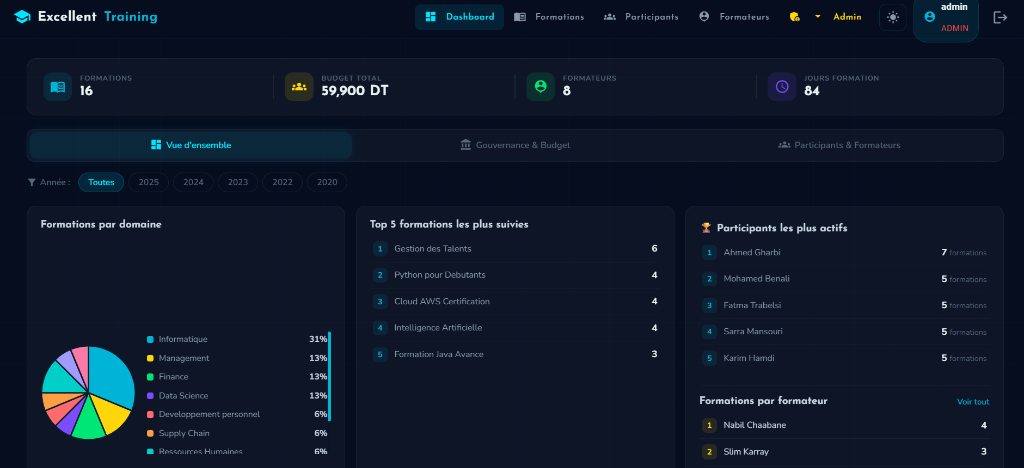
\includegraphics[width=\textwidth]{screenshots/img_dashboard_vue.png}
\caption{Dashboard Admin --- Onglet Vue d'ensemble : 4 cartes KPI (16 formations, 59900 DT, 8 formateurs, 84 jours), camembert par domaine, top 5 formations, participants les plus actifs et formateurs}
\label{fig:dash1}
\end{figure}

\begin{figure}[H]
\centering
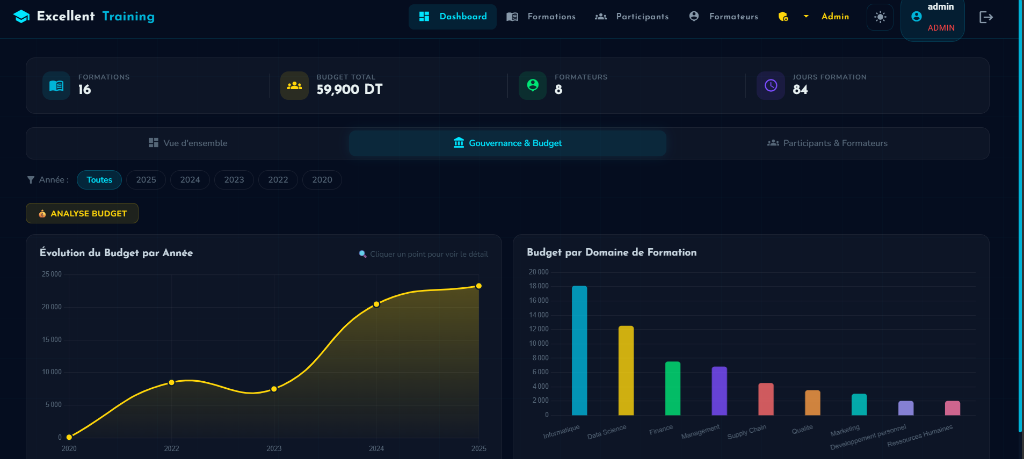
\includegraphics[width=\textwidth]{screenshots/img_dashboard_budget.png}
\caption{Dashboard Admin --- Onglet Gouvernance \& Budget : courbe d'\'{e}volution du budget par ann\'{e}e avec zoom interactif et barres par domaine}
\label{fig:dash2}
\end{figure}

\begin{figure}[H]
\centering
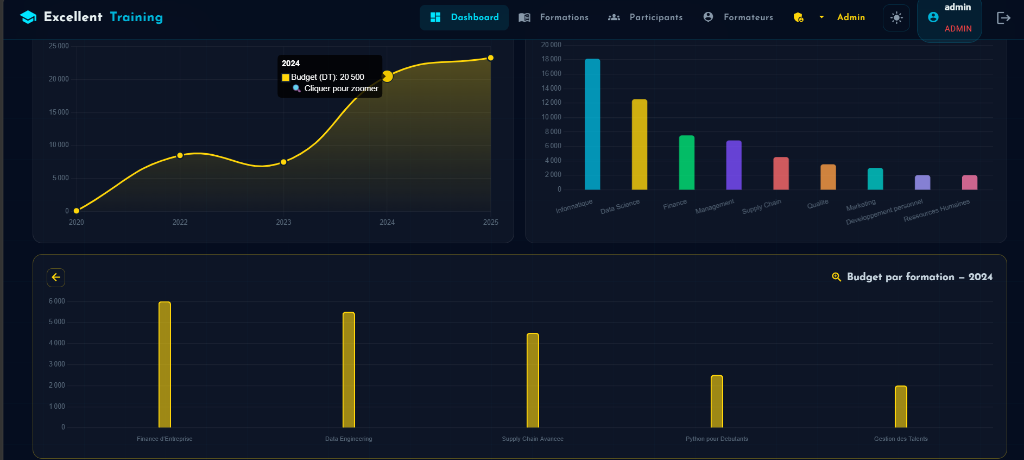
\includegraphics[width=\textwidth]{screenshots/img_dashboard_budget_zoom.png}
\caption{Dashboard --- Zoom interactif sur le budget 2024 : d\'{e}tail par formation avec barres verticales}
\label{fig:dash_budget_zoom}
\end{figure}

\begin{figure}[H]
\centering
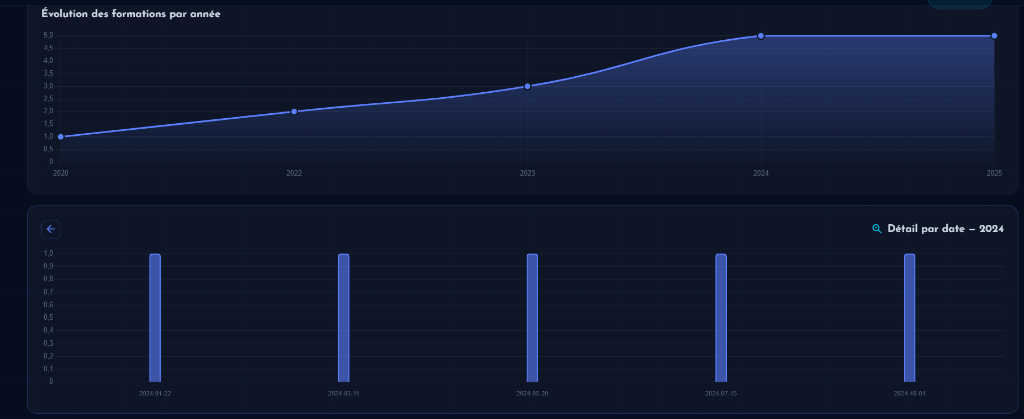
\includegraphics[width=\textwidth]{screenshots/img_dashboard_evolution.png}
\caption{Dashboard --- \'{E}volution des formations par ann\'{e}e avec zoom sur le d\'{e}tail par date (2024)}
\label{fig:dash_evolution}
\end{figure}

\begin{infobox}{Fonctionnalit\'{e}s du tableau de bord avanc\'{e}}
\begin{itemize}
  \item \textbf{3 onglets :} Vue d'ensemble, Gouvernance \& Budget, Participants \& Formateurs
  \item \textbf{Filtrage par ann\'{e}e :} Chips cliquables recalculant tous les pourcentages et classements dynamiquement
  \item \textbf{Zoom interactif :} Clic sur un point de courbe pour afficher le d\'{e}tail par formation
  \item \textbf{Top 5 participants actifs :} Classement par nombre de formations suivies
  \item \textbf{Top 5 formateurs :} Classement par nombre de formations dispens\'{e}es
  \item \textbf{Courbes avec remplissage :} Budget (jaune), participants (vert), formations (bleu)
\end{itemize}
\end{infobox}

\subsection{Barre de Navigation Admin}

La barre de navigation Admin comprend : Dashboard, Formations, Participants, Formateurs, menu Admin (en or) avec sous-menus : Domaines, Profils, Structures, Employeurs, Utilisateurs. Un toggle dark/light mode et les informations de l'utilisateur connect\'{e} sont affich\'{e}s \`{a} droite.

\begin{figure}[H]
\centering
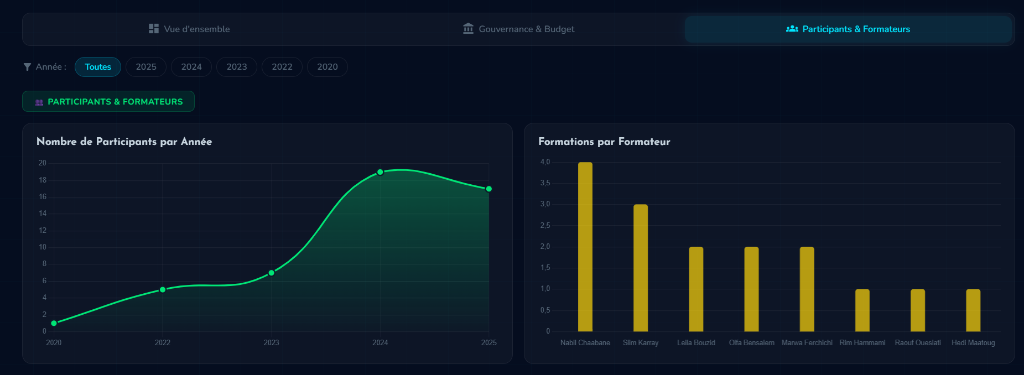
\includegraphics[width=\textwidth]{screenshots/img_dashboard_participants_formateurs.png}
\caption{Dashboard --- Onglet Participants \& Formateurs : courbe participants par ann\'{e}e et barres formations par formateur}
\label{fig:dash_part_form}
\end{figure}

\begin{figure}[H]
\centering
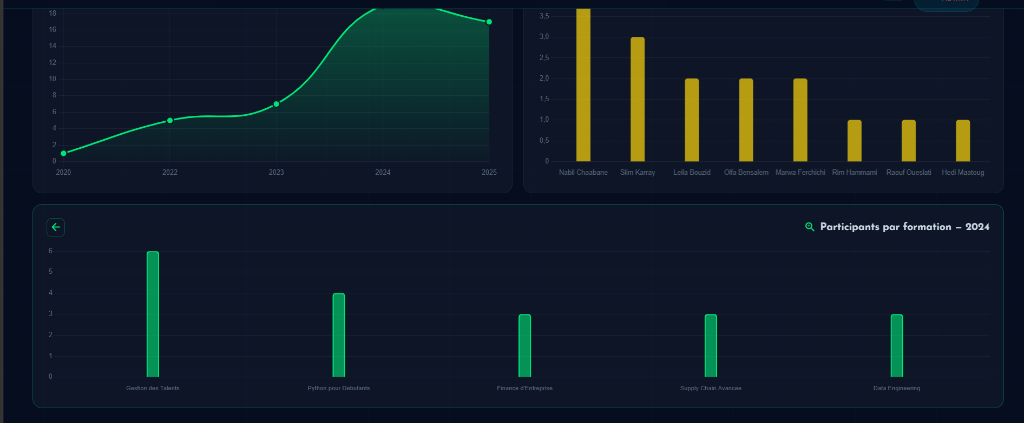
\includegraphics[width=\textwidth]{screenshots/img_dashboard_participants_zoom.png}
\caption{Dashboard --- Zoom participants par formation (2024) et d\'{e}tail formations par formateur}
\label{fig:dash_part_zoom}
\end{figure}

\clearpage
\section{Dashboard Responsable}

Le Responsable acc\`{e}de au m\^{e}me dashboard que l'Admin (statistiques, graphiques) mais sans le menu \textbf{Admin} en or dans la navbar.

\begin{notebox}{Diff\'{e}rence Admin vs Responsable}
Le Responsable voit le m\^{e}me dashboard que l'Admin (statistiques, graphiques) mais sans le menu \textbf{Admin} en or dans la navbar. Il n'a pas acc\`{e}s \`{a} la gestion des utilisateurs, domaines, structures, profils et employeurs.
\end{notebox}

\section{Interface Utilisateur Simple}

L'interface Utilisateur simple offre un acc\`{e}s limit\'{e} : ``Mes Formations'' (lecture seule), Formateurs et Participants. Pas de Dashboard ni de menu Admin.

\clearpage
\section{Anciennes Captures --- Formations, Participants, Formateurs}

\begin{figure}[H]
\centering
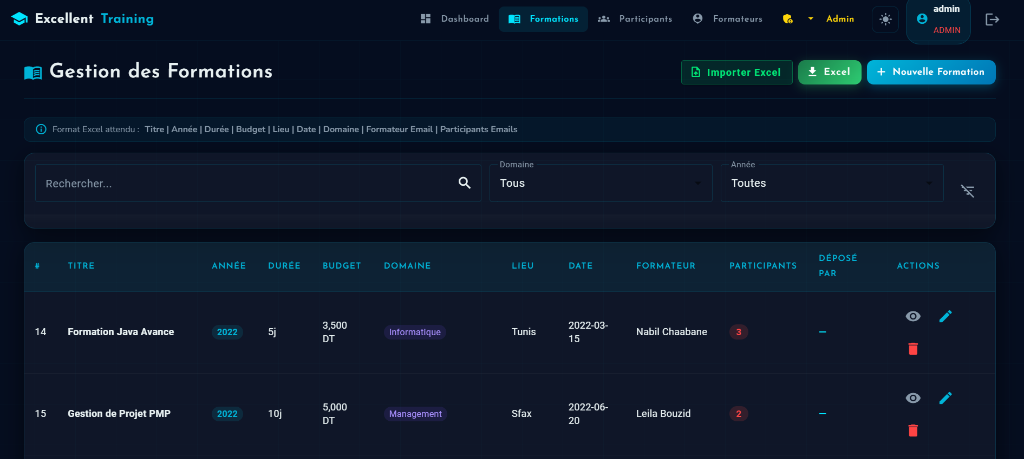
\includegraphics[width=\textwidth]{screenshots/img_formations_table_old.png}
\caption{Page Formations --- Tableau avec colonnes Titre, Ann\'{e}e, Dur\'{e}e, Budget, Domaine, Lieu, Date, Formateur, Participants, D\'{e}pos\'{e} par, Actions}
\label{fig:formations_old}
\end{figure}

\begin{figure}[H]
\centering
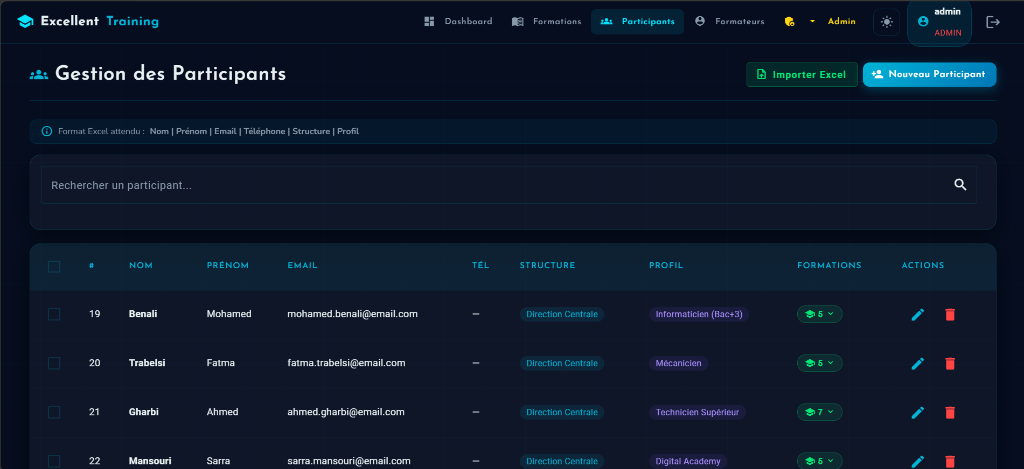
\includegraphics[width=\textwidth]{screenshots/img_participants_table_old.png}
\caption{Page Participants --- Tableau avec colonnes Nom, Pr\'{e}nom, Email, T\'{e}l, Structure, Profil, Formations (badge vert cliquable), Actions}
\label{fig:participants_old}
\end{figure}

\begin{figure}[H]
\centering
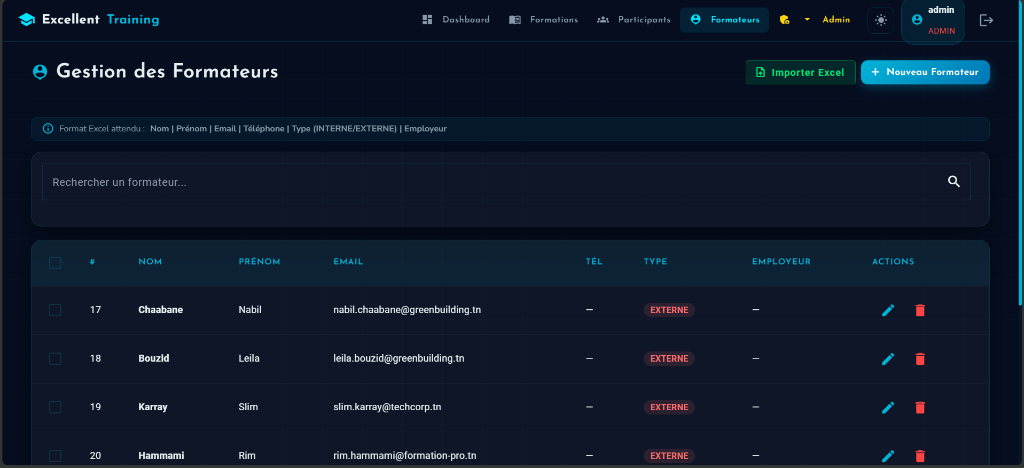
\includegraphics[width=\textwidth]{screenshots/img_formateurs_table_old.png}
\caption{Page Formateurs --- Tableau avec colonnes Nom, Pr\'{e}nom, Email, T\'{e}l, Type, Employeur, Actions}
\label{fig:formateurs_old}
\end{figure}

\begin{figure}[H]
\centering
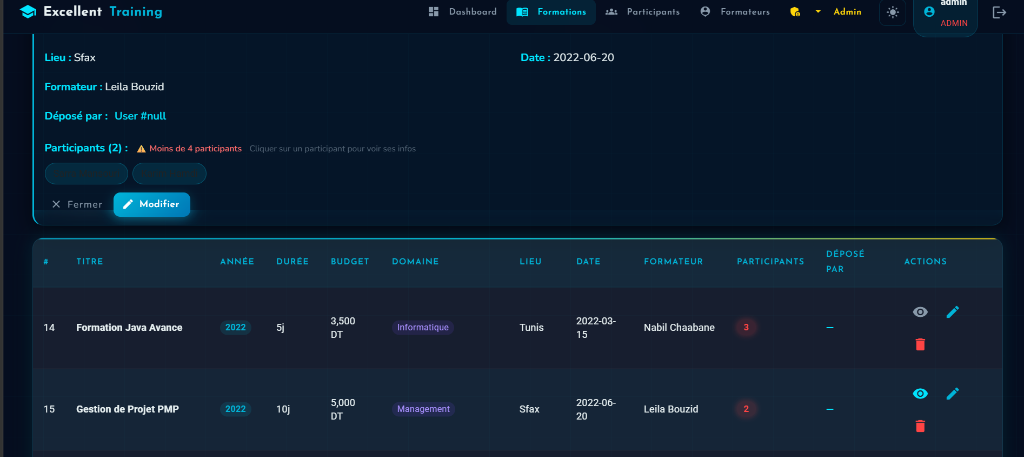
\includegraphics[width=\textwidth]{screenshots/img_formation_detail_old.png}
\caption{D\'{e}tail inline d'une formation --- Informations compl\`{e}tes avec participants, boutons Fermer et Modifier}
\label{fig:formation_detail_old}
\end{figure}

\begin{figure}[H]
\centering
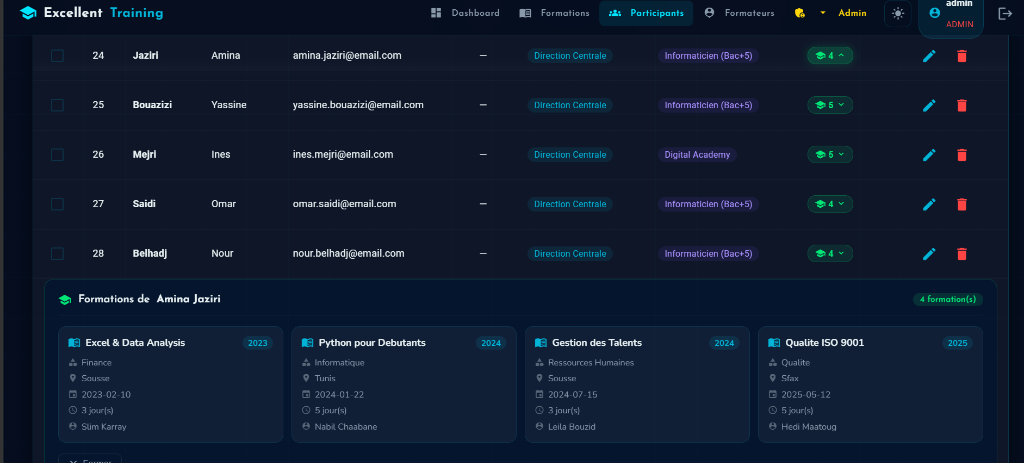
\includegraphics[width=\textwidth]{screenshots/img_participant_formations_old.png}
\caption{Formations d'un participant (Amina Jaziri) --- 4 formations affich\'{e}es inline sous la ligne}
\label{fig:participant_formations_old}
\end{figure}

\begin{successbox}{Contr\^{o}le d'acc\`{e}s c\^{o}t\'{e} interface}
\begin{itemize}
  \item \textbf{Navbar simplifi\'{e}e :} Seulement Mes Formations, Formateurs, Participants
  \item \textbf{Badge "Lecture seule" :} Affich\'{e} sur la page formations pour l'UTILISATEUR
  \item \textbf{Boutons contextuels :} "Nouvelle Formation" visible (ses propres formations) + Export Excel
  \item \textbf{Pas de Dashboard :} RoleGuard bloque l'acc\`{e}s et redirige vers /access-denied
  \item \textbf{Filtrage des donn\'{e}es :} L'UTILISATEUR ne voit que ses formations (\texttt{created\_by\_id})
\end{itemize}
\end{successbox}

\clearpage
\section{Gestion des Formations (Dark Mode)}

\begin{figure}[H]
\centering
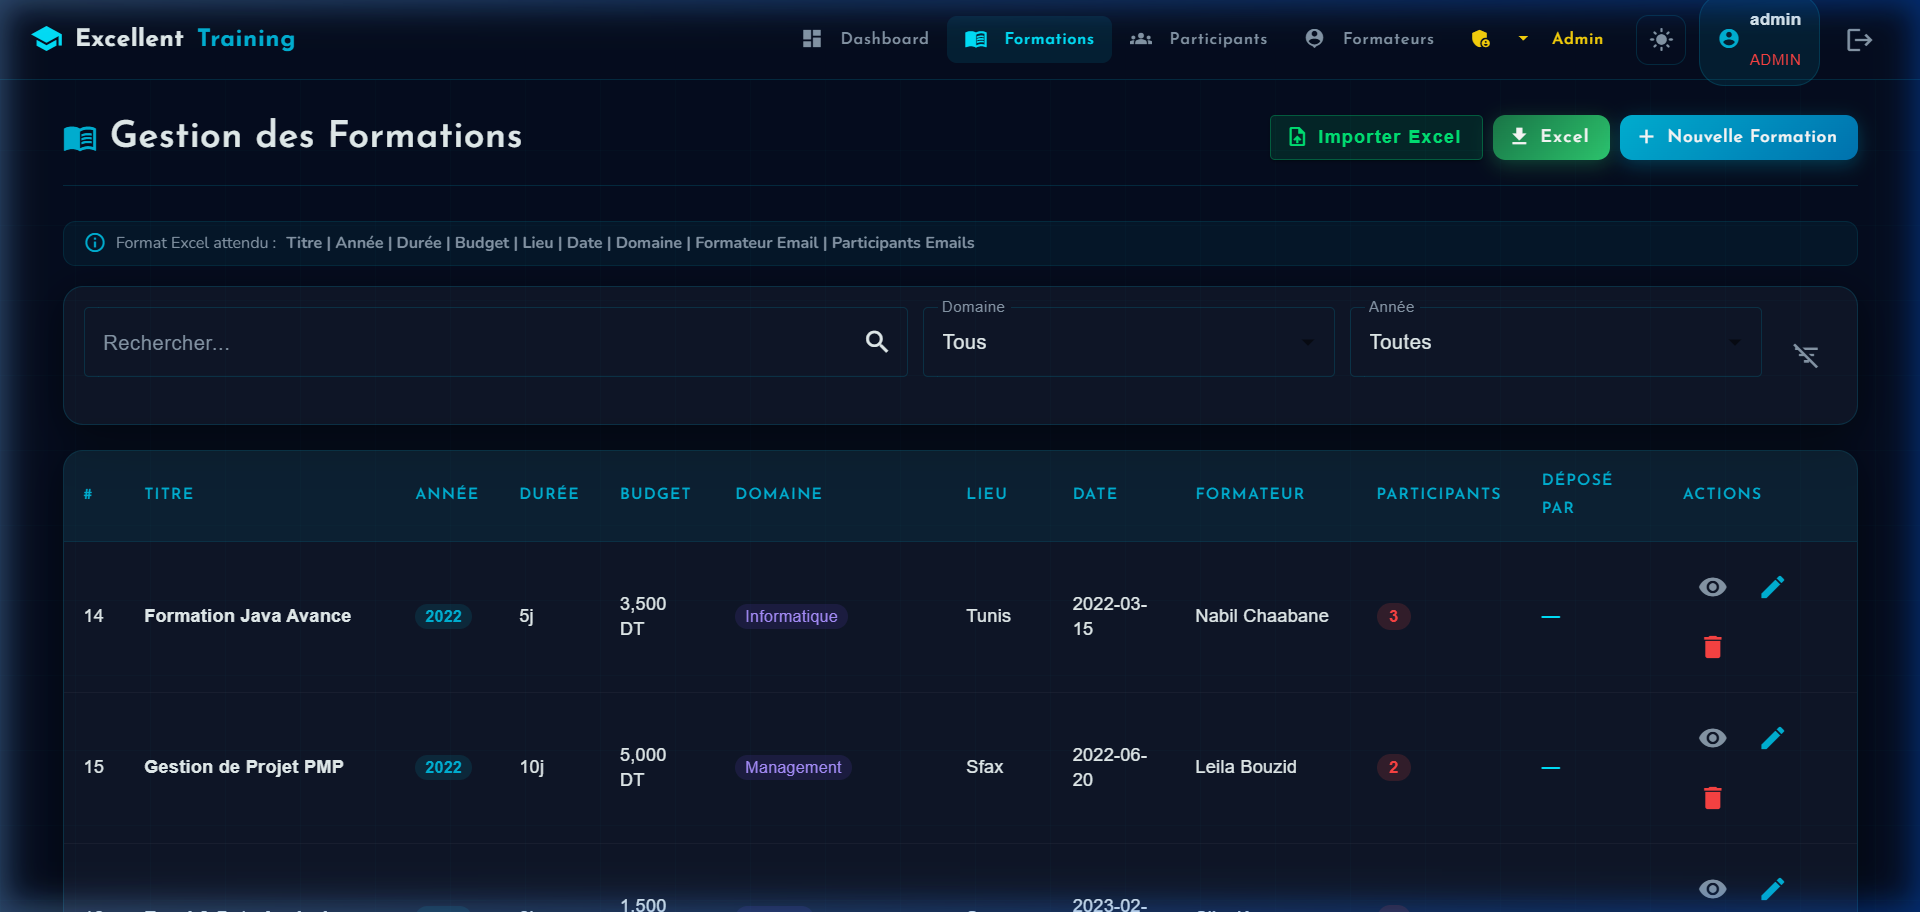
\includegraphics[width=\textwidth]{screenshots/formations_table.png}
\caption{Page Formations en dark mode --- Tableau complet avec colonnes Titre, Ann\'{e}e, Dur\'{e}e, Budget, Domaine, Lieu, Date, Formateur, Participants, D\'{e}pos\'{e} par et Actions}
\label{fig:formations_table}
\end{figure}

\subsection{D\'{e}tail Inline d'une Formation}

\begin{figure}[H]
\centering
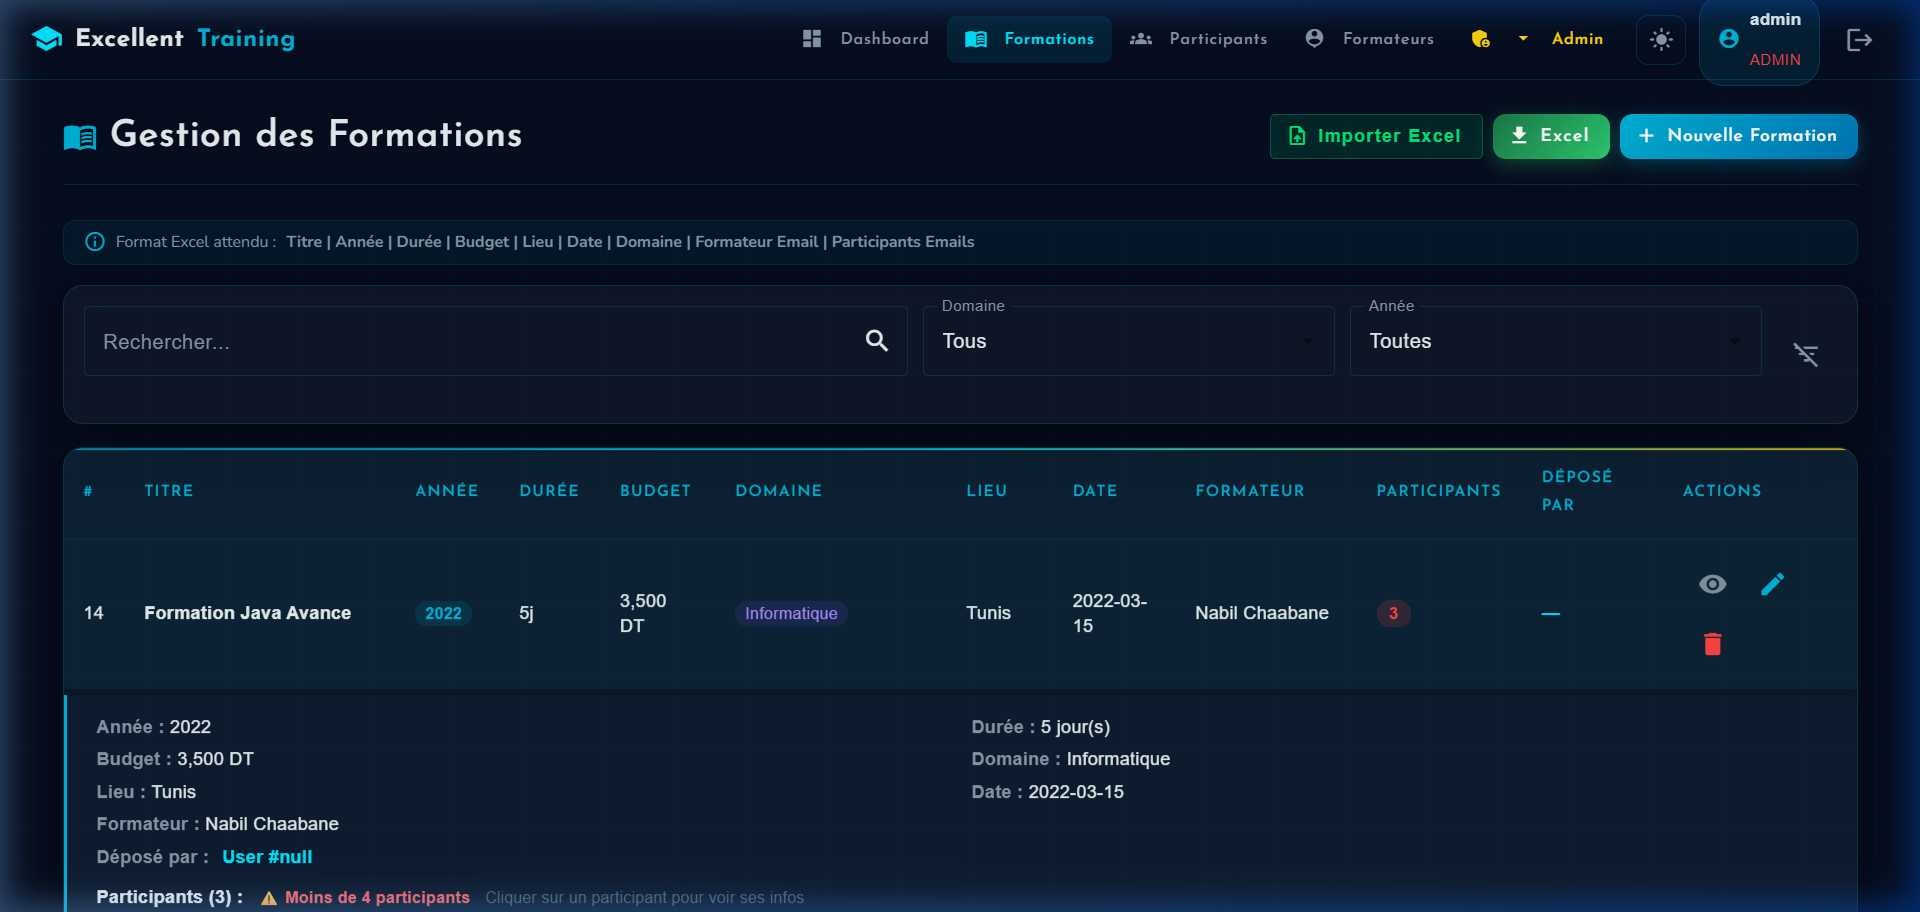
\includegraphics[width=\textwidth]{screenshots/formation_detail.png}
\caption{D\'{e}tail inline d'une formation --- Le panneau se d\'{e}ploie directement sous la ligne cliqu\'{e}e avec animation smooth (250ms)}
\label{fig:formation_detail}
\end{figure}

\begin{infobox}{Am\'{e}lioration UX : D\'{e}tail Inline}
Lors du clic sur l'ic\^{o}ne \textbf{Voir} (oeil), les informations d\'{e}taill\'{e}es de la formation s'affichent directement sous la ligne du tableau via la fonctionnalit\'{e} \texttt{multiTemplateDataRows} d'Angular Material. Cette approche \'{e}vite le d\'{e}filement vers le haut de la page et offre une exp\'{e}rience utilisateur fluide. Le panneau affiche : ann\'{e}e, dur\'{e}e, budget, domaine, lieu, date, formateur, d\'{e}pos\'{e} par, et la liste des participants sous forme de chips cliquables.
\end{infobox}

\clearpage
\section{Gestion des Participants (Dark Mode)}

\begin{figure}[H]
\centering
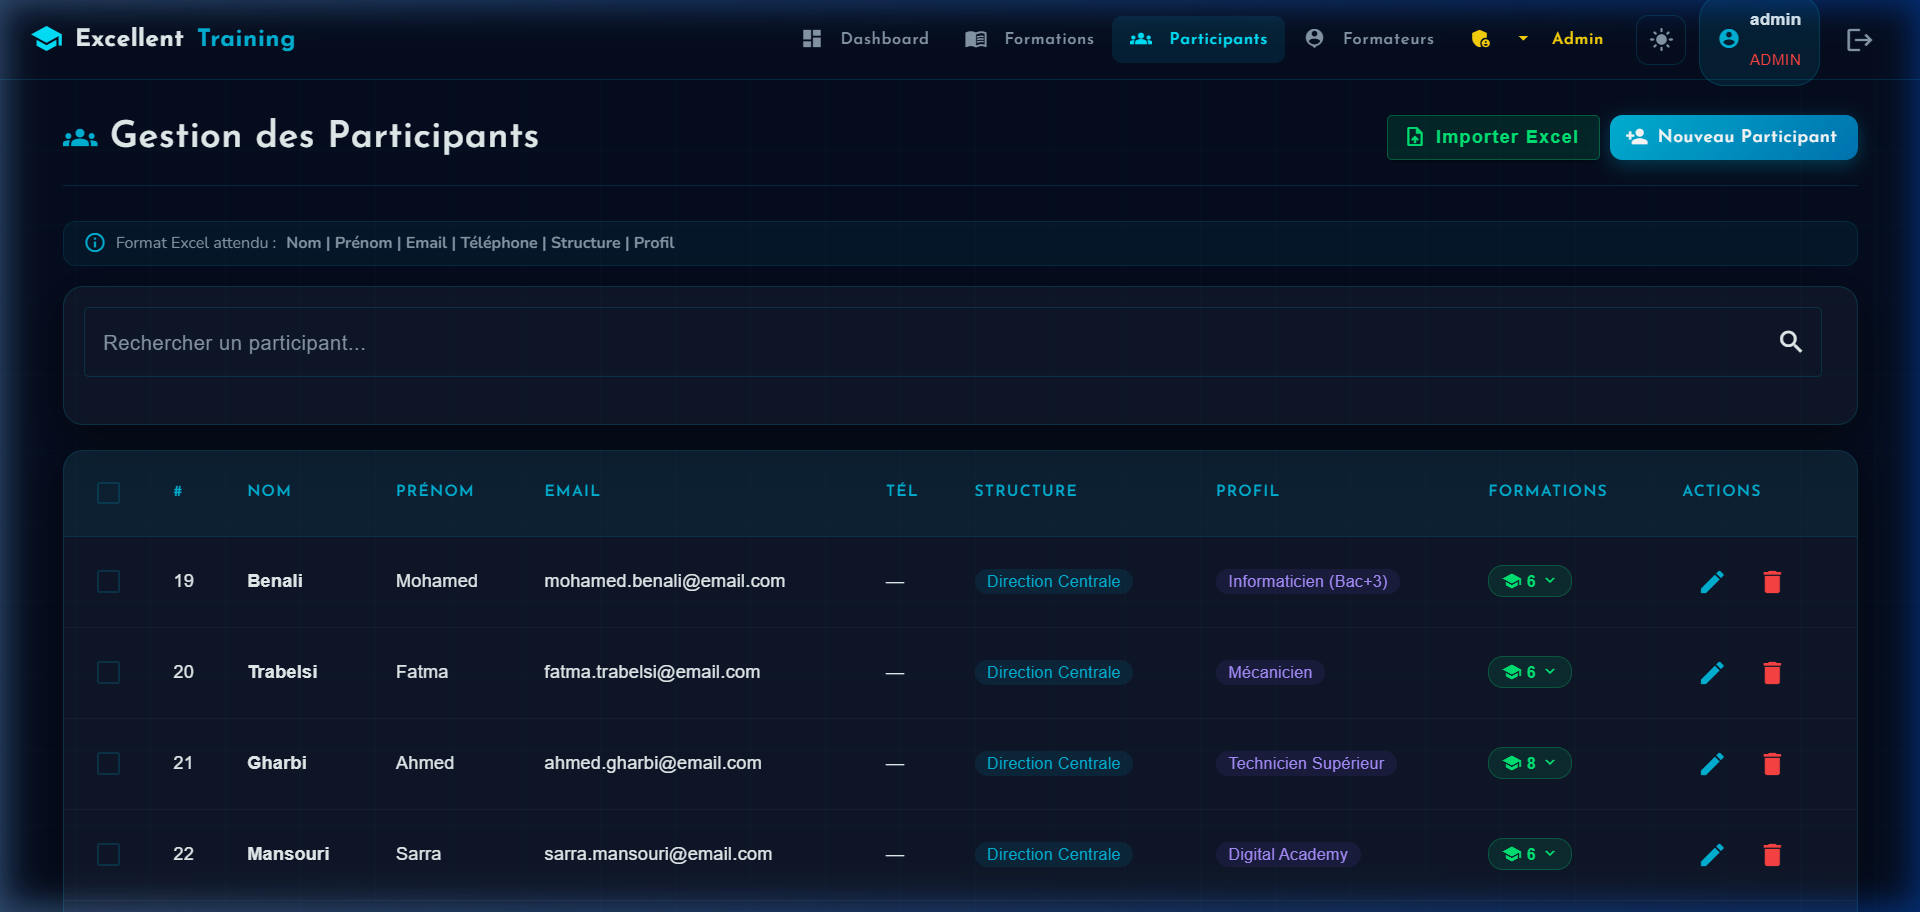
\includegraphics[width=\textwidth]{screenshots/participants_table.png}
\caption{Page Participants en dark mode --- Tableau avec colonnes Nom, Pr\'{e}nom, Email, T\'{e}l, Structure, Profil, Formations et Actions}
\label{fig:participants_table}
\end{figure}

\subsection{Formations d'un Participant (Inline)}

\begin{figure}[H]
\centering
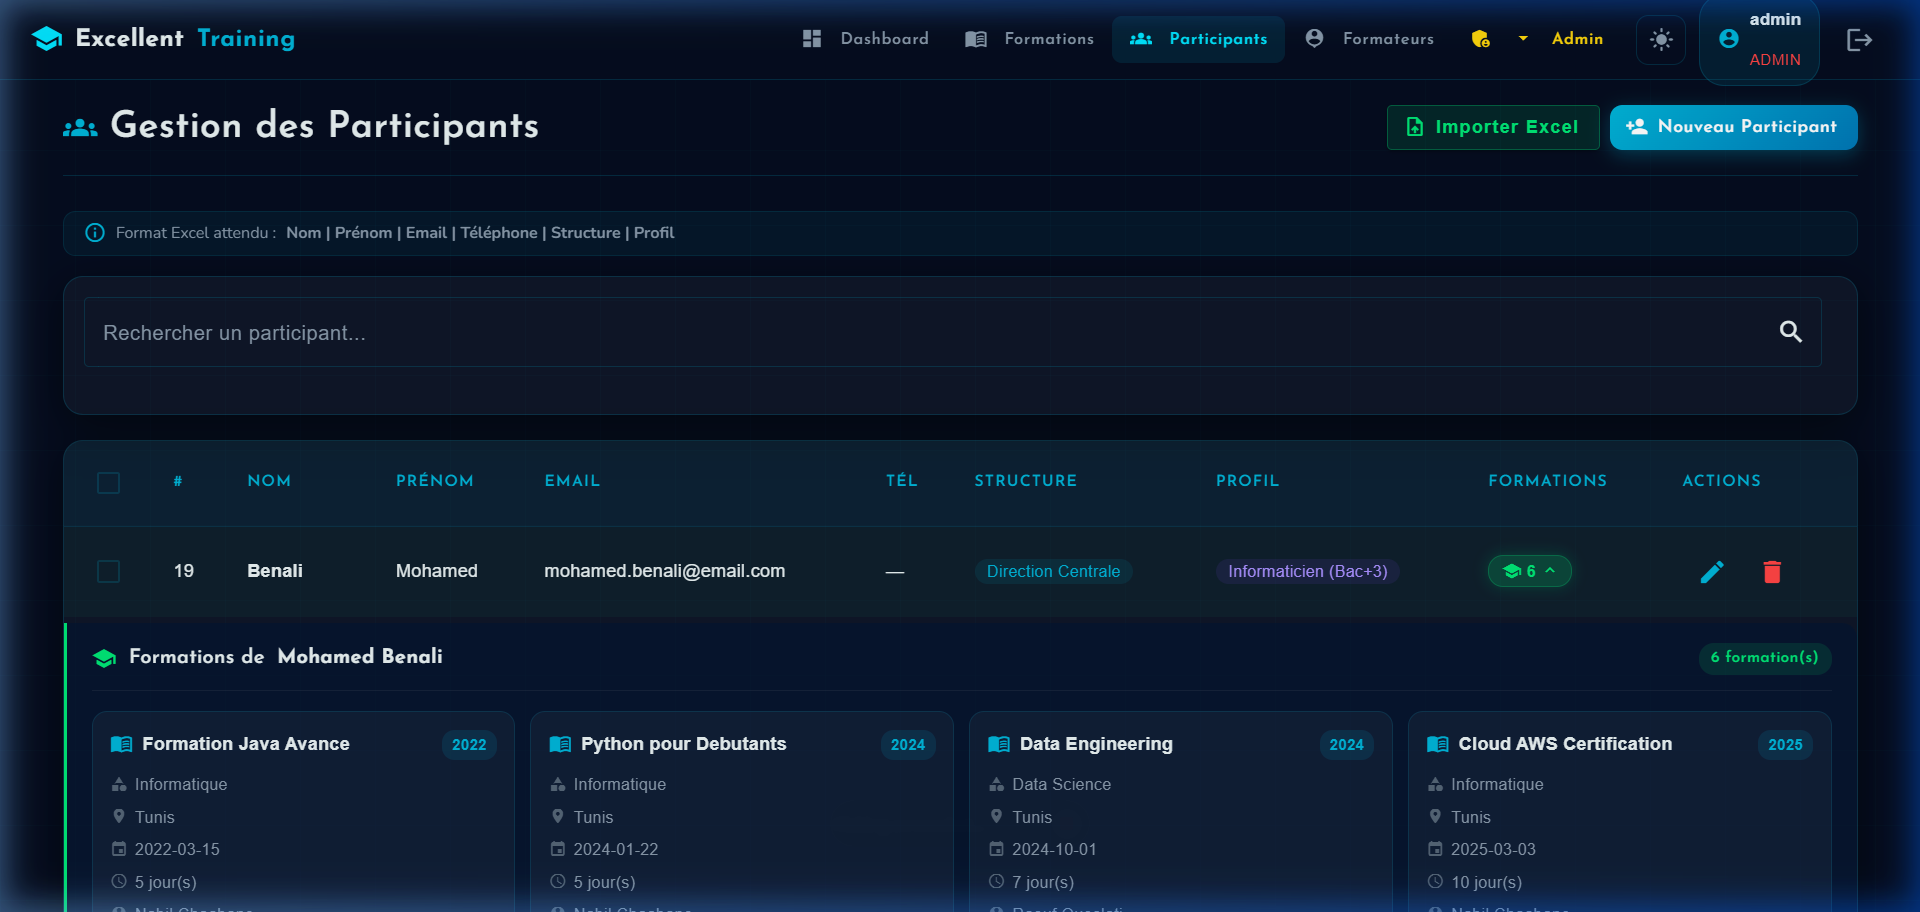
\includegraphics[width=\textwidth]{screenshots/participant_formations.png}
\caption{Formations du participant Mohamed Benali --- 6 formations affich\'{e}es dans des cartes inline sous la ligne cliqu\'{e}e}
\label{fig:participant_formations}
\end{figure}

\begin{infobox}{Formations associ\'{e}es \`{a} un participant}
En cliquant sur le badge vert \textbf{Formations} d'un participant, un panneau inline s'ouvre sous la ligne avec toutes les formations auxquelles ce participant est inscrit. Chaque formation est affich\'{e}e dans une carte avec : titre, ann\'{e}e, domaine, lieu, date, dur\'{e}e et formateur. L'animation \texttt{@detailExpand} assure une transition fluide.
\end{infobox}

\clearpage
\section{Gestion des Formateurs (Dark Mode)}

\subsection{Formations d'un Formateur (Nouvelle Fonctionnalit\'{e})}

\begin{figure}[H]
\centering
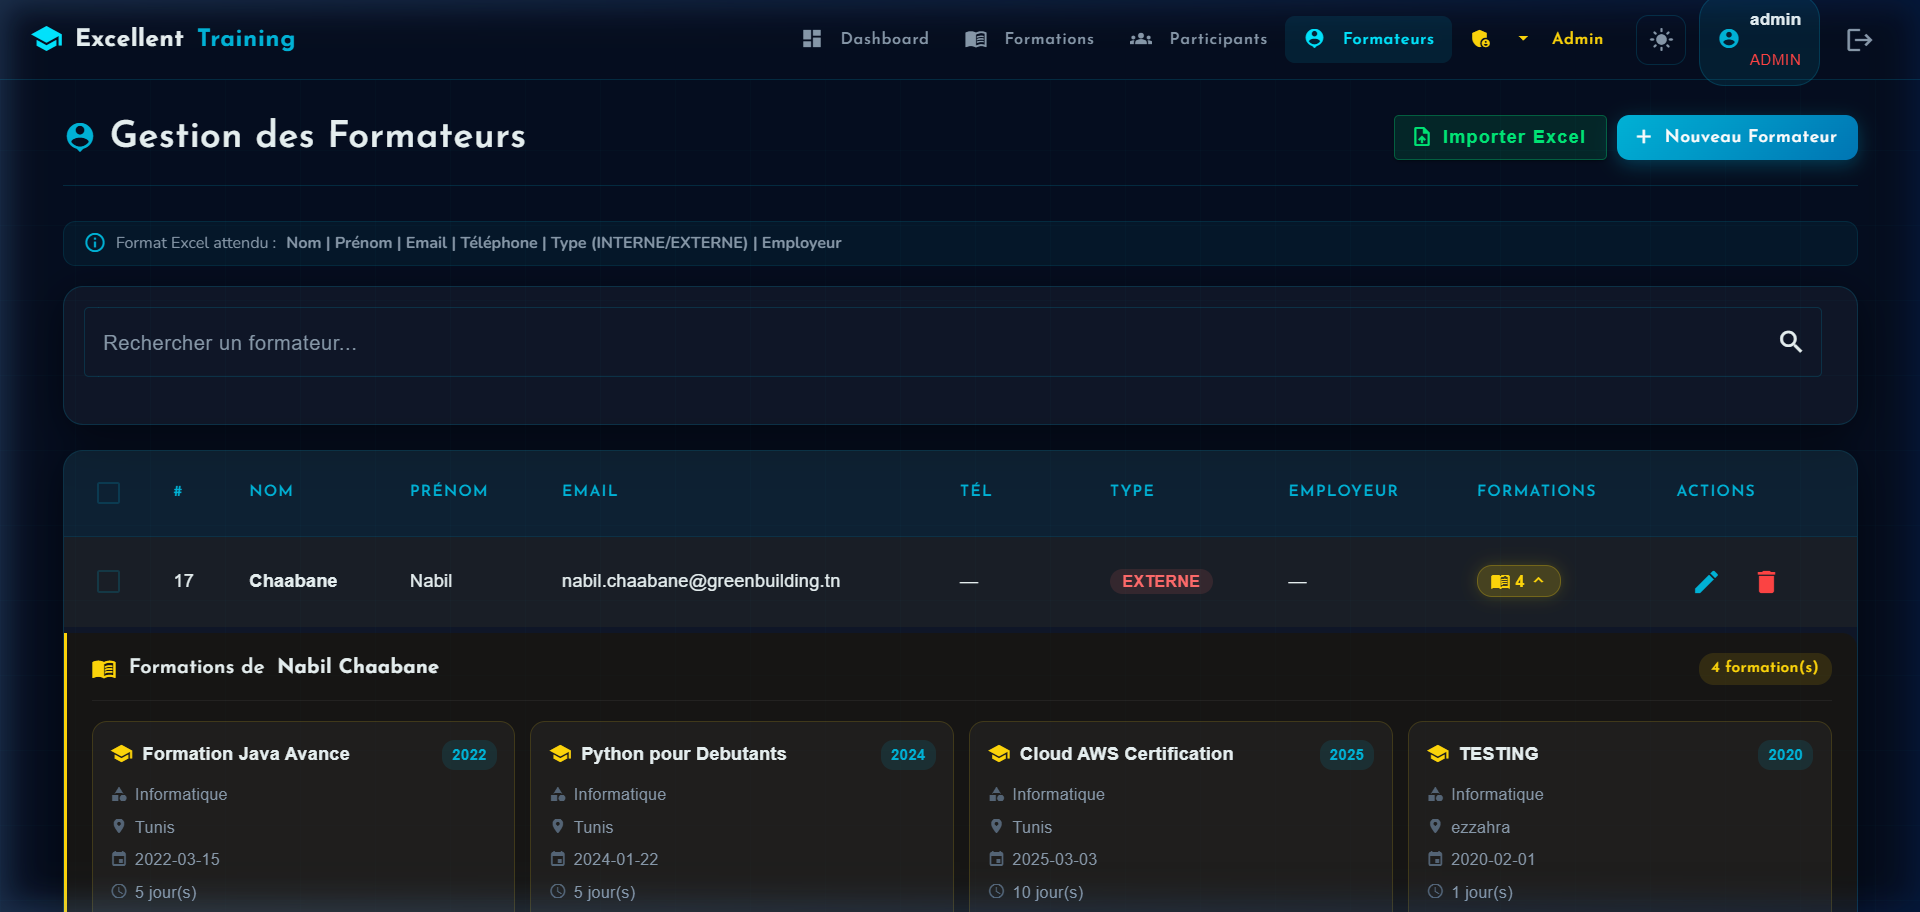
\includegraphics[width=\textwidth]{screenshots/formateurs_formations.png}
\caption{Formateurs avec colonne Formations --- Le formateur Nabil Chaabane dispense 4 formations, affich\'{e}es inline sous sa ligne}
\label{fig:formateurs_formations}
\end{figure}

\begin{successbox}{Nouvelle fonctionnalit\'{e} : Formations par formateur}
Une nouvelle colonne \textbf{Formations} a \'{e}t\'{e} ajout\'{e}e au tableau des formateurs. Elle affiche un badge dor\'{e} avec le nombre de formations dispens\'{e}es. Au clic, un panneau inline s'ouvre montrant les d\'{e}tails de chaque formation (titre, ann\'{e}e, domaine, lieu, date, dur\'{e}e, nombre de participants). Cette fonctionnalit\'{e} exploite le m\^{e}me m\'{e}canisme \texttt{multiTemplateDataRows} utilis\'{e} pour les formations et les participants.
\end{successbox}

\clearpage
\section{Dashboard Avanc\'{e} (Dark Mode)}

\begin{figure}[H]
\centering
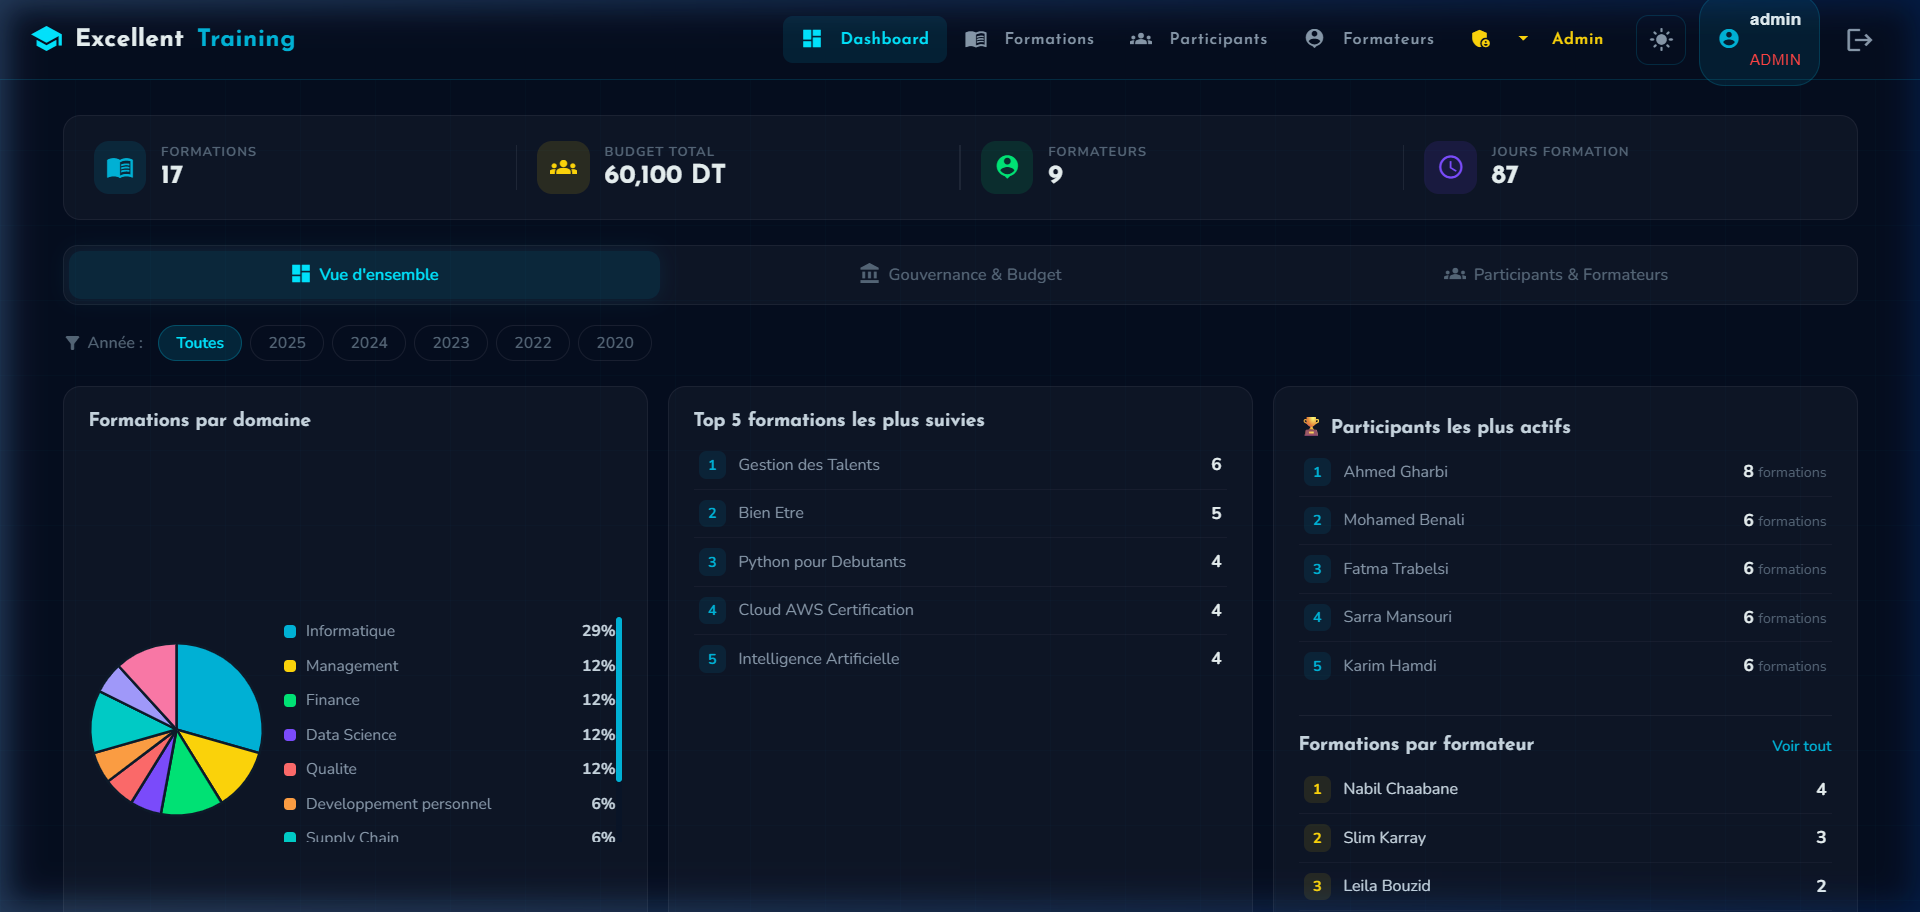
\includegraphics[width=\textwidth]{screenshots/dashboard.png}
\caption{Dashboard Admin en dark mode --- Vue d'ensemble avec 4 cartes KPI, camembert par domaine, Top 5 formations, participants actifs et formations par formateur}
\label{fig:dashboard_dark}
\end{figure}

% ??????????????????????????????????????????????????????
\chapter{Conclusion}
% ??????????????????????????????????????????????????????

\section{Bilan du Projet}

Ce projet a permis de r\'{e}aliser une application web compl\`{e}te r\'{e}pondant \`{a} toutes les exigences du cahier des charges \cite{cdc2026}, avec plusieurs fonctionnalit\'{e}s suppl\'{e}mentaires allant au-del\`{a} des sp\'{e}cifications initiales. Les principaux acquis sont :

\begin{itemize}
  \item Ma\^{\i}trise de l'architecture \textbf{Spring Boot} : entit\'{e}s JPA, repositories, services, controllers REST
  \item Impl\'{e}mentation d'une \textbf{s\'{e}curit\'{e} JWT} robuste avec gestion des r\^{o}les (RBAC)
  \item D\'{e}veloppement d'une \textbf{SPA Angular} avec navigation prot\'{e}g\'{e}e par guards
  \item Mise en place de \textbf{contr\^{o}les de saisie} \`{a} deux niveaux (frontend + backend)
  \item \textbf{Import/Export Excel} : import en masse de formations, participants et formateurs avec cr\'{e}ation automatique des entit\'{e}s li\'{e}es ; export format\'{e} via Apache POI
  \item \textbf{Suppression en lot} : multi-s\'{e}lection avec checkboxes pour suppression group\'{e}e de participants et formateurs
  \item \textbf{Dashboard avanc\'{e}} : 3 onglets (Vue d'ensemble, Gouvernance \& Budget, Participants \& Formateurs) avec filtrage par ann\'{e}e, zoom interactif sur les courbes, top 5 participants les plus actifs et top formateurs
  \item \textbf{D\'{e}tail inline (multiTemplateDataRows)} : les informations d\'{e}taill\'{e}es des formations, participants et formateurs s'affichent directement sous la ligne cliqu\'{e}e, sans d\'{e}filement de page, avec animation smooth
  \item \textbf{Formations par formateur} : nouvelle colonne affichant les formations dispens\'{e}es par chaque formateur avec expansion inline
  \item \textbf{Recherche en temps r\'{e}el} : filtrage instantan\'{e} sur tous les champs dans les pages formations, participants et formateurs
  \item Design moderne avec \textbf{dark/light mode} et animations CSS
  \item Int\'{e}gration de \textbf{reCAPTCHA v2} et \textbf{v\'{e}rification email} via Gmail SMTP
\end{itemize}

\section{Perspectives d'Am\'{e}lioration}

\begin{itemize}
  \item G\'{e}n\'{e}ration de rapports PDF automatiques (JasperReports ou iText)
  \item Notifications en temps r\'{e}el lors d'ajout de formations (WebSocket)
  \item Application mobile compl\'{e}mentaire (React Native ou Ionic)
  \item D\'{e}ploiement sur cloud (Docker + AWS/Azure) avec pipeline CI/CD
  \item Tests unitaires et d'int\'{e}gration automatis\'{e}s (JUnit + Karma/Jasmine)
  \item Gestion des \'{e}valuations post-formation et certification
\end{itemize}

\vspace{1cm}
\begin{successbox}{D\'{e}p\^{o}t GitHub du projet}
  \small\url{https://github.com/oussema-abdelmoumen/Gestion-Formation-Excellent-Training}\\[4pt]
  \footnotesize Stack : Spring Boot 3.2 \textbullet{} Angular 17 \textbullet{} MySQL 8 \textbullet{} JWT \textbullet{} BCrypt \textbullet{} Apache POI \textbullet{} reCAPTCHA v2
\end{successbox}

% ??? BIBLIOGRAPHIE ????????????????????????????????????
\begin{thebibliography}{9}
  \bibitem{cdc2026} Institut Sup\'{e}rieur d'Informatique.
    \textit{Cahier des charges --- Mini-Projet 2026 : Conception et d\'{e}veloppement d'une application de gestion de formation}.
    ISI Tunis El Manar, 2025.

  \bibitem{springboot} Spring Framework Documentation.
    \textit{Spring Boot Reference Documentation 3.2.x}.
    Pivotal Software, 2024. \url{https://docs.spring.io/spring-boot/docs/3.2.x/reference/html/}

  \bibitem{angular17} Google.
    \textit{Angular Documentation v17}.
    Google, 2024. \url{https://angular.io/docs}

  \bibitem{jwt} Auth0.
    \textit{JSON Web Tokens --- Introduction}.
    Auth0, 2024. \url{https://jwt.io/introduction}

  \bibitem{springsec} Spring Security Documentation.
    \textit{Spring Security Reference 6.2}.
    Pivotal, 2024. \url{https://docs.spring.io/spring-security/reference/}

  \bibitem{poi} Apache Software Foundation.
    \textit{Apache POI --- the Java API for Microsoft Documents}.
    Apache, 2024. \url{https://poi.apache.org/}

  \bibitem{bcrypt} Provos N., Mazi\`{e}res D.
    \textit{A Future-Adaptable Password Scheme}.
    USENIX Annual Technical Conference, 1999.

  \bibitem{recaptcha} Google.
    \textit{reCAPTCHA v2 Developer Guide}.
    Google Cloud, 2024. \url{https://developers.google.com/recaptcha/docs/display}

  \bibitem{hibernate} Red Hat.
    \textit{Hibernate ORM 6.3 User Guide}.
    Red Hat, 2024. \url{https://docs.jboss.org/hibernate/orm/6.3/}
\end{thebibliography}

\end{document}
